\cotefile{150}

\scanpage{52}
Je veux revenir sur la condition b), qui peut se préciser beaucoup, si on veut utiliser à fond l'information qu'on avait dans le numéro précédent.

$b_1)$ Pour $x\in\Sigma\deleted{\unsure{(0)}}=\Sigma^{\unsure{*|<}}(0)$, les $z_\alpha\in\Sigma^{<}(1)$ au dessus de $x$ (pour l'application \uline{but} : $\Sigma^{<}(1)\overset{\uline{b}}{\unsure{-|\longrightarrow}}\Sigma^{<}(0)$) sont en correspondance biunivoque avec les germes \inserted{$B_\alpha$} en $x$ de sous-espaces bordants de $\Sigma^{<}(0)$, \deleted{\unsure{avec}} images par $\uline{b}$ des germes de $\Sigma^{<}(1)$ en \deleted{\unsure{les}} $z_\alpha$.

$b_2)$ \deleted{Il existe un} Si $n=\operatorname{card}(\{z_\alpha\})$, il existe un élément \deleted{\unsure{d}} unique de $\Sigma^{<}(n)$, soit $\widetilde{x}$, tel que les \deleted{$\unsure{B_\alpha|z_\alpha}$} $z_\alpha$ soient les images de $\widetilde{x}$ par \inserted{les $n$ applications} de $\widetilde\Sigma(n)$ dans $\widetilde\Sigma(1)$.
\margin{\diagram{\begin{tikzcd}[column sep=large]
\unsure{\widetilde\Sigma^{<}(n)}\arrow[r,phantom,"{\substack{\cdot\\\cdot}}"{description,pos=0.26,yshift=-2.5ex}]\arrow[r,shift left=2ex,"\varphi_{0,n}"]\arrow[r,"\varphi_{1,n}" description]\arrow[r,shift right=2ex,"\varphi_{n-1,n}"']&\widetilde\Sigma^{*}(1)\arrow[d,phantom,"{\rotatebox{90}{$\in$}}" description]\\
&z_\alpha
\end{tikzcd}}}
(Il en résulte qu'il y a une \uline{structure d'ordre} \inserted{\uline{total}} \uline{naturelle} sur l'ens des ``strates de niveau 1'' $B_\alpha$ \inserted{dans $\Sigma^{<}(0)=\Sigma$} passant par $x$)

\deleted{\unsure{$b_2)$}} $b_3)$ Pour tout \deleted{$1\leq d\leq n$, \unsure{les}} $1\leq d\leq n$, considérons l'application
\[
\Sigma^{<}(d)\underset{\substack{\inserted{\text{imm}}\\\deleted{\unsure{\text{vigueur}}}}}{\longrightarrow}\underset{\substack{\rotatebox{90}{$\in$}\\x}}{\Sigma^{<}(0)}
\]
associée à l'inclusion \deleted{\unsure{de de}} $\{d\}\subset\{0,1,--,d\}$, les pts \inserted{$z$} de $\Sigma^{<}(d)$ au dessus de $x$ sont en correspondance biunivoque avec l'ens des parties \inserted{de card $d$} de un \deleted{$\unsure{\Sigma}$} $I$ des germes $B_\alpha$, ou encore l'ens des parties \inserted{de card $d$} de l'ens $I$ des $z_\alpha$, ou encore avec $\mathcal P_d([0,--,n-1])$, en associant : à telle partie $A$ l'application \inserted{str} croissante unique de $\Delta_d=\{0,--d\}$ en

% Lighter-hand foliation at the lower-left corner, not authorial numbering.
\margin{\handwritten{51}}

\scanpage{53}
\mspage{22}
$\Delta_n=\{0,-,n\}$ dont l'image soit $A\cup\{n\}$, et l'hom simplicial correspondant
\diagram{\begin{tikzcd}[column sep=small]
\Sigma^{<}(n)\arrow[r,hook,"\mathrm{imm}"]\arrow[d,phantom,"{\rotatebox{90}{$\in$}}" description]&\Sigma^{<}(d)\arrow[d,phantom,"{\rotatebox{90}{$\in$}}" description]&\deleted{\unsure{(\longrightarrow}}&\big(\arrow[r,dashed,"\mathrm{imm}"]&\Sigma^{<}(0)\big)\arrow[d,phantom,"{\rotatebox{90}{$\in$}}" description]\\
\widetilde x&z\ \deleted{\unsure{z}}&&&x
\end{tikzcd}}
\diagram{\begin{tikzcd}
\deleted{x}\arrow[r,phantom,"\deleted{\longleftarrow}" description]&\deleted{\unsure{\Sigma(0)}}
\end{tikzcd}}
et l'image de $\widetilde x$ par celui-ci. De plus, pour $z$ dans \deleted{ainsi} $\Sigma^{<}(d)$ au dessus de $x$, $\deleted{\unsure{Z|z}}$ le germe de sous-espace de $\Sigma^{<}(0)$ en $x$, image du germe de $\Sigma^{<}(d)$ en $z$, est juste l'intersection des germes $B_\alpha$ \unsure{correspondant|correspondants} aux $z_\alpha\in A$.

On s'intéresse ici aux morphismes entre les $\Sigma^{<}(n)$ correspondant aux applications strictement croissantes d'ens. tot\textsuperscript{t} ordonnés non vides $d\hookrightarrow d'$ tel que $d$ soit cofinal dans $d'$. La catégorie de ces objets et morphismes équivaut à celle des ens tot. ordonnés $d$ (év.\textsuperscript{t} vides), par le foncteur qui à un tel $d$ associe $d\coprod\{\omega\}$, où $\omega$ est un ``dernier élément'', et à tout $d'\hookrightarrow d$ str. croiss le prolongement par $\omega\mapsto\omega$. On a donc \deleted{\unsure{$\Sigma$}} un foncteur
\[
\Gamma:d-\Sigma^{<}(d\coprod\{\omega\})
\]
sur les ens \unsure{tot.|tot} ordonnés év.\textsuperscript{t} vides, dont la
% Cancelled interline beneath « donnée équivaut à celle… »; its attachment/revision order is not established.
\begin{tabular}[t]{@{}l@{}}
donnée équivaut à celle des $\Sigma^{<}(n)$ avec les\\
\deleted{\unsure{qui équivaut à}}
\end{tabular}
appl. simpliciales ``cofinales'' entre eux. Et la donnée d'\deleted{F}un tel foncteur $\Gamma$ revient à la donnée de $\Gamma(\varnothing)$ (ici $\Sigma^{\unsure{*|<}}(0)$) et
% Pale pencil foliation at the lower left, in another hand.
\margin{52}

\scanpage{54}
d'un objet (espace) simplicial --- \uline{dessus de}
$\Gamma(\varnothing)=\Sigma^{<}(0)$. Ici il s'agit d'un espace
\margin{NB $\Gamma(n)=\Sigma^{*}(n+1)$}
simplicial relatif, et les conditions $b_1,b_2,b_3$
concernent cette structure --- elles disent
essentiellement que cette structure est associée
à une stratification cylindrique locale de
$\Sigma^{<}(0)=\Sigma$, et ``ordonnée'' (i.e. l'ens des
strates de codim $1$ passant par un $x\in\Sigma$ sont
\deleted{\unsure{est}} \unsure{ordonnés|ordonnées}, et cette relation d'ordre varie
continûment avec $x$ en un sens évident).

Les \deleted{$\Sigma^{<}(d)$ \unsure{s'id|s'ident}} $\Gamma(d)$\inserted{$=\Sigma^{<}(d+1)$} s'identifient alors
aux \deleted{parties} espaces des \inserted{(germes de)} strates de codim
$d+1$, \deleted{les} \inserted{germes} identifiés \deleted{(grâce à la structure
d'ordre)} aux ens de germes de strates
de codim $1$ \deleted{\unsure{de}} \inserted{\unsure{en un}} $=$ $x$. Les applic\unsure{ns}
semi-simpliciales entre les $\Gamma(d)$ proviennent
alors de la structure d'ordre --- \deleted{\unsure{on y}}
\unsure{pour|peut} réconstituer les espaces de drapeaux
associés à la stratification, à l'aide des
\deleted{\unsure{cette|ces}} $\Gamma(d)$, grâce à cette structure ordonnée.
En résumé, la donnée de $\Gamma:d\mathrel{\mid\! -\!}\Gamma(d)$
\deleted{\unsure{i.e. de}} (i.e. de $\Sigma^{<}$ avec les \unsure{ap|app} \unsure{semi|\deleted{semi}} simpliciales
cofinales) équivaut à celle d'un $\Sigma=\Sigma^{<}(0)$,
\margin{53}

\scanpage{55}
\mspage{23}
avec la structure de stratification cylindrique \inserted{ordonnée}
locale. \deleted{Par exemple}, Une autre façon de
décrire les $\Gamma(d)=\Sigma^{<}(d+1)$, c'est de
prendre la puiss. \deleted{\unsure{sym.}} \inserted{cart. relative} $d$.ième de $\Gamma_0$\deleted{\unsure{$(\varnothing)$}}\inserted{$=\Sigma^{<}(1)$}
sur $\Sigma\ (=\Gamma(\varnothing))$, dont on enlève les images
des puiss. cart. relatives \deleted{\unsure{inférieures}} \inserted{\deleted{$\Gamma'(d)$} des $d'$.ième ($d'<d$)} par les applic\unsure{ns}
$\tfrac12$ simpliciales entre celles ci. Cela donne à priori
les \deleted{\unsure{ens tot.}} suites ordonnées de $d$ germes de
strates de codim $1$ \inserted{en un $=$ point,} \unsure{(mutuel\textsuperscript{t}|\deleted{(mutuel\textsuperscript{t}}} distinctes), \deleted{soit}
$\Gamma'(d)$. On a alors \inserted{$\unsure{\Gamma^{\deleted{'}}(d)|\Gamma(d)}\subset\Gamma'(d)$},
$\Gamma(d)$ est une partie à la fois ouverte et
\unsure{fermée|\deleted{fermée}} de $\Gamma'(d)$, et \deleted{$\Gamma'(d)\unsure{\simeq}$}
\[
(35)\qquad \Gamma'(d)\simeq\unsure{\mathfrak S_d|\mathcal S_d}\times\Gamma(d)
\]
Pour avoir \deleted{la}\inserted{une} structure d'ordre \inserted{total} relative, de
\margin{\deleted{il s'agit de}}
\deleted{\unsure{$\Gamma'(1)$ sur}} $\Gamma_0=\Sigma^{<}(1)$ sur $\Sigma_{\deleted{\unsure{*|0}}}=\Sigma^{<}(0)$, il \deleted{suffit}\inserted{\unsure{uniquement}}
de se donner, \deleted{dans $\Gamma'_1(\unsure{0|2})=\unsure{\Sigma^{<}(0)|\Sigma^{<}(2)}$, $\Gamma'_{1+1}$} dans
$\Gamma_0\times_\Sigma\Gamma_0\setminus\text{diagonale}$, une partie \inserted{(i.e. \unsure{néc.}} ouverte et fermée)
$\Gamma_1$, telle que $\Gamma_1\cup{}^s\Gamma_1=\Gamma_0\times\Gamma_0\setminus\text{diag}$, $\Gamma_1\cap{}^s\Gamma_1=\varnothing$
\margin{$\Gamma_1$ est le graphe de la relation $x<y$}
i.e. une section de $\Gamma_0\times_\Sigma\Gamma_0\setminus\text{diag}$ \unsure{au|\deleted{au}} dessus
\margin{ou une section \deleted{de $\Gamma_0\times_\Sigma\Gamma_0\setminus\unsure{\text{diagonale}|\text{diag}}$}\deleted{de $\operatorname{Sym}^2(\Gamma_0\times_\Sigma\Gamma_0)$}\deleted{de}}
de $\operatorname{Sym}^2_\Sigma(\Gamma_0)^*$ (``choix d'un premier élément parmi deux
éléments distincts), avec la condition de transitivité
\deleted{$\unsure{\text{que }\Gamma_1}$}
\diagram{\begin{tikzcd}[column sep=large,row sep=small]
(36)\quad (\Gamma_1\times_\Sigma\Gamma_0)\cap(\Gamma_0\times_\Sigma\Gamma_1)
 \arrow[r,"{\unsure{\operatorname{Pr}|\mathrm{P}}_{\unsure{13|23}}}"] \arrow[d,phantom,"\cap" description]
 & \Gamma_0\times\Gamma_0 \arrow[d,phantom,"\cup" description]
 & \text{se factorise par }\Gamma_1 \\
\unsure{\Sigma_0|\Gamma_0}\times\Gamma_0\times\Gamma_0 & \Gamma_1 &
\end{tikzcd}}
\margin{54}

\scanpage{56}
Je m'aperçois finalement que j'ai
pas mal bousillé pour arriver à trouver des
formulations simples --- car j'ai \uline{mélangé} des
propriétés purement ensemblistes de l'ens ordonné
$\Sigma=\Sigma^{<}(0)$, avec \unsure{\deleted{leur}|leur} interprétation semi-simpliciale,
et \deleted{\unsure{leur} \illegible{1}}\inserted{les} aspects topologiques. Je \uline{reprends}

\deleted{$\Sigma$ ens.}
% Detached pen marks, without a secure textual function: [307,869,327,885],
% [350,877,369,884], [422,886,459,901]; isolated stroke [939,773,949,790].
$\underset{\substack{\Vert\\\Sigma(0)}}{\Sigma}$ ens ordonné, muni d'une topologie \deleted{séparée}\inserted{(pour}
Si $\Sigma_1$ est le graphe de la relation d'ordre, on suppose

\textcircled{a} $\Sigma(1)\xrightarrow{\uline{b}\unsure{=|:}\operatorname{pr}_2}\Sigma(0)$ est propre et loc. immersif bordant
\unsure{\inserted{(propriétés topologiques)}|(propriétés topologiques)} \deleted{Cela implique}

\deleted{\textcircled{b}} \deleted{que l'applic\unsure{ati|ation}}
Cela implique que l'application diagonale est
ouverte, donc si $\Sigma$ séparé, son image est une
partie à la fois ouverte et fermee --- et on
peut alors introduire $\Sigma_F^{\unsure{<|*}}(1)=\Sigma(1)\setminus\text{diagonale}$.
Si $\Sigma$ est séparé, la propreté de $\Sigma(1)-\Sigma(0)$
implique aussi que $\Sigma_1$ est \uline{fermé} dans \deleted{$\Sigma(0)\times\Sigma(0)$}\inserted{$\Sigma\times\Sigma$}.

\textcircled{b} Pour tt $x\in\Sigma$, l'ens \inserted{(fini)} $\Sigma_{\leq x}$ \inserted{(fibre de $x$ dans $\Sigma(1)$)} est \uline{tot. ordonné}
pour l'ordre induit.
\deleted{\textcircled{\unsure{c}}} Donc la donnée d'un drapeau \inserted{$x_{i_0}-x_{\unsure{j_d|i_d}}$} de longueur
$d$ dans $\Sigma_\leq$ équivaut à celle d'une partie de card. $d+1$

% Lighter-hand foliation at the lower-left corner.
\margin{\handwritten{55}}

\scanpage{57}
\mspage{24}
de l'ens à $N(x)+1$ éléments, où $N(x)=\operatorname{card}(\Sigma_{\unsure{<|\leq}x})$.
Ou encore, si on regarde l'application-but
\[
\Sigma^{<}(d)\longrightarrow\unsure{\Sigma}=\Sigma^{<}(0)
\]
\[
(x_0<-<x_d)\longmapsto x_d
\]
la fibre de $x\in\Sigma$ s'identifie à l'ens \deleted{des parties}
$\unsure{\mathfrak P|\mathcal P}_d(\{1,.-,N(x)\})$.
La structure relative de $\Sigma^{\unsure{<|*}}(1)$ sur $\Sigma=\Sigma^{<}(0)$
% Isolated dark written sign directly below the bare middle Sigma, between
% this line and the next: two short forked left strokes joined to a compact
% loop or oval at the right. Identity and mathematical attachment unassigned.
\illegible{1}
est donc celle d'un ens tot. ordonné relatif, qui
permet de reconstituer le système des $\Sigma^{*}(d)$
\deleted{avec} $(d\in\mathbb N)$ avec les applications semi-simpliciales
correspondant aux morphismes cofinaux entre
les ens tot. ordonnés-types.
% Slanted marginal note beside the preceding three lines; its words are
% not an insertion after semi-simpliciales. The final circled character is unclear.
\margin{Tout ceci est donc à faire indépendt de toute condition topologique \unsure{\textcircled{a}}.}

\textcircled{c} $\forall\ x\in\Sigma$, les germes \inserted{$B_\alpha$} de sous-espaces \inserted{bordants} de $\Sigma$ en $x$
correspondants, par \unsure{\textcircled{a}}, aux $z_\alpha\in\Sigma^{\unsure{<|*}}(1)$ au dessus
de $x$ (par $\Sigma^{\unsure{<|*}}(1)\overset{\underline b}{\unsure{-|\longrightarrow}}\Sigma$) sont mutuellement transver-
saux (et à fortiori distincts).
Les germes intersections de certains des $B_\alpha$
correspondent donc aux pts des $\Sigma^{\unsure{<|*}}(d)$ au dessus
de $x$ (par $\Sigma^{\unsure{<|*}}(d)\overset{\underline b}{\relbar\joinrel\relbar}\Sigma$), comme
images du \deleted{\unsure{dit}} germe de $\Sigma^{\unsure{<|*}}(d)$ en ces pts.
% Separate cancelled small looped glyph immediately before Les; no letter assigned.
\deleted{\illegible{1}} Les espaces $\Sigma^{*}(d)$ $(d\in\mathbb N)$ et les
applications $\tfrac12$ simpliciales cofinales entre eux, \deleted{\unsure{satisfa}}
% In the preceding cancellation a small final loop follows the tall f;
% its reading as a remains doubtful, and the abandoned word is not completed.
ou encore l'espace relatif $\Sigma^{\unsure{<|*}}(1)$ sur $\Sigma^{<}(0)$ et la
structure d'ordre relative, est décrit entièrement
% Pale bottom-left foliation, apparently another hand; the top authorial number is 24.
\margin{56}

\scanpage{58}
par $\Sigma$, muni d'une stratification locale
cylindrique ordonnée : $\Sigma'(1)$ est l'espace des
strates de codim $1$, $\Sigma'(1)\overset{\uline{b}}{-}\Sigma\unsure{{}_{0}|.}$ l'application
associant à un germe son centre, $\Sigma'(2)$ est
l'espace des paires de germes $B,B'$ en $x$
\deleted{\unsure{que}} tels que : $\{B\}<\{B'\}$ \unsure{\illegible{1}..|...}
\margin{\diagram{\begin{tikzcd}[
  row sep={1.3cm,between origins},
  column sep=0pt,
  cells={nodes={anchor=center}},
  /tikz/execute at end picture={
    % D1--D4: four disconnected continuation components, relative to N1.
    \draw[line width=.35pt]
      ([xshift=-2mm,yshift=12mm]scan058top.center)--
      ([xshift=-1.8mm,yshift=11mm]scan058top.center);
    \draw[line width=.35pt]
      ([xshift=-1.8mm,yshift=9.5mm]scan058top.center)--
      ([xshift=-1.8mm,yshift=8.3mm]scan058top.center);
    \draw[line width=.35pt]
      ([xshift=-1.6mm,yshift=6.9mm]scan058top.center)--
      ([xshift=-1.6mm,yshift=6.1mm]scan058top.center);
    \draw[line width=.35pt]
      ([xshift=-1.4mm,yshift=4.6mm]scan058top.center)--
      ([xshift=-1.2mm,yshift=3.4mm]scan058top.center);
  }
]
% N1: alias adds only an invisible coordinate name.
|[alias=scan058top]| \Sigma^{\unsure{<|*}}(2)
\arrow[from=1-1,to=2-1,
  /tikz/arrows=->,/tikz/>=stealth,/tikz/line width=.4pt,
  /tikz/shorten >=0pt,/tikz/shorten <=0pt,
  to path={
    ([xshift=-4mm,yshift=-3mm]\tikztostart.center)--
    ([xshift=-4mm,yshift=3mm]\tikztotarget.center)
    node[midway,right] {$\uline{s}'$}\tikztonodes
  }]
\arrow[from=1-1,to=2-1,
  /tikz/arrows=->,/tikz/>=stealth,/tikz/line width=.4pt,
  /tikz/shorten >=0pt,/tikz/shorten <=0pt,
  to path={
    ([xshift=3mm,yshift=-3mm]\tikztostart.center)--
    ([xshift=3mm,yshift=3mm]\tikztotarget.center)
    node[midway,right] {$\uline{b}'$}\tikztonodes
  }]
\\
% N2: exact accepted label and unsure scope.
\unsure{\Sigma^{<}(1)|\Sigma^{*}(1)}
\arrow[from=2-1,to=3-1,
  /tikz/arrows=->,/tikz/>=stealth,/tikz/line width=.4pt,
  /tikz/shorten >=0pt,/tikz/shorten <=0pt,
  to path={
    ([xshift=-4mm,yshift=-2.5mm]\tikztostart.center)--
    ([xshift=-4mm,yshift=3mm]\tikztotarget.center)
    node[midway,right] {$\uline{b}$}\tikztonodes
  }]
\\[-.1cm]
% N3: exact accepted label.
\Sigma=\Sigma^{\unsure{<|*}}(0)
\end{tikzcd}}}
Pour retrouver la relation d'ordre sur $\Sigma\unsure{=|\substack{-\\0}}\Sigma^{\unsure{<|*}}(0)$
\inserted{à partir de la structure d'ordre relative $\Sigma^{\unsure{*|<}}(1)$ sur $\Sigma^{<}(0)$ (celle
qui \unsure{place} $\Sigma^{<}(1)$ pour les relations strictes $x<y$)}
il faut donc de plus se donner une application
continue
\[
(36)\qquad\Sigma^{<}(1)\overset{\uline{s}\unsure{=|:}p_1}{-}\Sigma_{\deleted{\unsure{*|\varnothing|0}}}=\Sigma^{<}(0)
\]
qui soit injective \deleted{et croissante} sur chaque fibre \inserted{$\uline{b}^{-1}(x)$}
de $\Sigma^{<}(1)\overset{\uline{b}}{-}\Sigma_{\deleted{\unsure{*|\varnothing|0}}}$ (i.e. $\Sigma^{<}(1)\overset{(\uline{s},\uline{b})}{-}\Sigma\times\Sigma$ inj.)
et d'image $\not\ni x$ (i.e. $\operatorname{Im}(\uline{s},\uline{b})\cap\operatorname{diag}(\Sigma\times\Sigma)=\varnothing$)

\deleted{et on doit se donner de plus
\[
(37)\qquad\Sigma^{<}(2)\xrightarrow{\unsure{\varphi_2|p_2}}\Sigma^{*}(1)\quad(\hookrightarrow\Sigma\times\Sigma
\]
\margin{NB la donnée de $\unsure{\varphi_2|p_2}$ équivaut à celle des deux composés
$\operatorname{pr}_{\unsure{0|1}}\circ\varphi;\operatorname{pr}_{\unsure{1|2}}\circ\varphi:\Sigma^{<}(2)\rightrightarrows\Sigma$
qu'on \unsure{se} donne}
\margin{inutile de se donner $p_2$, il est déterminé ($v\ p_1$), cf \unsure{pg} suivante\unsure{.-|..|...}}
\[
(38)\qquad
\Sigma^{<}(2)\xrightarrow{(\operatorname{pr}_1\circ\varphi,\operatorname{pr}_2\circ\varphi,\unsure{\Psi|\psi})}\Sigma_0\times\Sigma_0\times\Sigma_0
\]
\unsure{\deleted{Dont}|Dont} l'image est par construction (voir \unsure{\deleted{$\varphi$}|$\varphi$|\illegible{1}} (37))
dans $\Sigma_1\times\Sigma_0$ et dans
}
\margin{\handwritten{57}}

\scanpage{59}
\mspage{\unsure{\{25\}}}
de telle façon qu'il existe
\[
(37)\qquad p_2:\Sigma^{<}(2)\longrightarrow\Sigma^{\unsure{<|*}}(1)
\]
tel que
\[
(38)\qquad \left\{\begin{aligned}
\uline{b}\circ p_2&=\uline{s}\circ\uline{b'}\\[6em]
p_1\circ p_2&=p_1\circ\uline{s'}
\end{aligned}\right.
\]
i.e. le carré
\diagram{\begin{tikzcd}[row sep=large,column sep=large,name=s59square,execute at end picture={
\coordinate (s59ha) at ([xshift=10pt]s59sourcea.east);
\fill ([yshift=6pt]s59ha) circle[radius=.45pt];
\draw[line width=.7pt,line cap=round] ([xshift=-1.5pt,yshift=5.5pt]s59ha)--([xshift=-2.5pt,yshift=5pt]s59ha);
\draw[line width=.7pt,line cap=round] ([xshift=-3pt,yshift=4.3pt]s59ha)--([xshift=-3.4pt,yshift=3.4pt]s59ha);
\draw[line width=.7pt,line cap=round] ([xshift=-3.8pt,yshift=2.7pt]s59ha)--([xshift=-3.7pt,yshift=2pt]s59ha);
\draw[line width=.7pt,line cap=round] ([xshift=-3.2pt,yshift=1.2pt]s59ha)--([xshift=-2.6pt,yshift=.4pt]s59ha);
\coordinate (s59hb) at ([xshift=10pt]s59sourceb.east);
\fill ([yshift=6pt]s59hb) circle[radius=.45pt];
\fill ([xshift=-1.8pt,yshift=6.1pt]s59hb) circle[radius=.5pt];
\fill ([xshift=-3.7pt,yshift=4.7pt]s59hb) circle[radius=.55pt];
\fill ([xshift=-4.8pt,yshift=3.2pt]s59hb) circle[radius=.55pt];
\draw[line width=.8pt,line cap=round] ([xshift=-5pt,yshift=1.3pt]s59hb)--([xshift=-4.2pt,yshift=.3pt]s59hb);
\fill ([yshift=4pt]s59targetd.north) circle[radius=.9pt];
}]
|[alias=s59sourcea]|\Sigma^{<}(2)\arrow[r,"\uline{b'}",start anchor=east,shorten <=10pt]\arrow[d,"p_2"] & \Sigma^{<}(1)\arrow[d,"p_1=\uline{s}",dash,end anchor=north,shorten >=4pt]\\
|[alias=s59sourceb]|\Sigma^{<}(1)\arrow[r,"\uline{b}",start anchor=east,shorten <=10pt] & |[alias=s59targetd]|\Sigma
\arrow[ul,phantom,"\text{(cart)}" description]
\end{tikzcd}}
commutatif
\figure{\begin{tikzpicture}[x=1cm,y=1cm]
\draw[line width=.45pt,line cap=round] (0,0)
.. controls (.65,-.02) and (.90,.02) .. (1.08,.13)
-- (1.30,.50)
.. controls (1.55,.72) and (1.70,.77) .. (1.90,.76)
.. controls (2.70,.70) and (3.50,.81) .. (4.90,.77);
\end{tikzpicture}}

i.e. le carré
\diagram{\begin{tikzcd}[name=s59diamond,execute at end picture={
\coordinate (s59hc) at ([xshift=-6pt,yshift=6pt]s59sourcec.north west);
\draw[line width=.7pt,line cap=round] ([xshift=-4.5pt,yshift=2pt]s59hc)--([xshift=-4.2pt,yshift=1pt]s59hc);
\draw[line width=.7pt,line cap=round] ([xshift=-2.8pt]s59hc)--([xshift=-1.7pt,yshift=-.2pt]s59hc);
\fill (s59hc) circle[radius=.5pt];
\draw[line width=.7pt,line cap=round] ([xshift=2pt,yshift=.8pt]s59hc)--([xshift=2.8pt,yshift=1.5pt]s59hc);
}]
& \Sigma^{<}(1)\arrow[dl,"p_1"'] & \\
\Sigma && |[alias=s59sourcec]|\Sigma^{<}(2)\arrow[ul,"\uline{s'}"',start anchor=north west,shorten <=7pt]\arrow[dl,"p_2"]\\
&\Sigma^{<}(1)\arrow[ul,"p_1"]&
\end{tikzcd}}
est comm.

Ce qui détermine $p_2$ de façon unique, puisque
$(\deleted{\unsure{b}},p_1,\uline{b}):\Sigma^{<}(1)\unsure{\longrightarrow|\mathrel{-}}\Sigma\unsure{<|\times}\Sigma$ est mono).
De plus, on \deleted{\unsure{suppose}}\inserted{doit} exiger que le premier carré
(38) soit \uline{cartésien}, et que $p_1:\Sigma^{<}(1)\unsure{\longrightarrow|\mathrel{-}}\Sigma$
est \uline{transversal} p.r. à l'immersion bordante
$\uline{b}:$ \diagram{\begin{tikzcd}[column sep=large,execute at end picture={
\coordinate (s59hi) at ([xshift=9pt]s59inline.east);
\draw[line width=.65pt,line cap=round] ([yshift=6pt]s59hi)--([xshift=-1.4pt,yshift=5.8pt]s59hi);
\draw[line width=.65pt,line cap=round] ([xshift=-3pt,yshift=5pt]s59hi)--([xshift=-4.2pt,yshift=4.3pt]s59hi)--([xshift=-5pt,yshift=2.8pt]s59hi)--([xshift=-4.4pt,yshift=1.3pt]s59hi)--([xshift=-3pt,yshift=.4pt]s59hi);
\fill ([xshift=-1.5pt]s59hi) circle[radius=.4pt];
}]
|[alias=s59inline]|\Sigma^{<}(1)\arrow[r,"\uline{b}",start anchor=east,shorten <=9pt]&\Sigma
\end{tikzcd}} (ce qui est \deleted{\unsure{une}}\inserted{l'unique} condition de
nature non purement algébrique\ldots)
Posons alors, pour $x,y\in\Sigma$
\[
(39)\qquad x\prec y\quad\Longleftrightarrow\quad\exists\ u\in\Sigma_{<}(1)\text{ tel que }x=p_1u,\ y=\uline{b}u
\]
\margin{58}

\scanpage{60}
On voit alors que
\[
x\prec y\text{ et }y\prec z\quad\Longrightarrow\quad x\prec z
\]
car soient $u,v\in\Sigma_{\unsure{<|*}}(1)$ tels que
\[
\mathord{\rlap{$\deleted{\unsure{s}}$}p}_1 u=x,\quad\uline{b}u=\underbrace{y,\quad p_1}v=y,\quad\uline{b}v=z
\]
% In the first glyph the possible cancelled s overlaps the head of p;
% the earlier letter is unresolved. The short brace is spatial: it lies
% beneath the first y toward the following p_1, not beneath both complete equalities.
on a donc
\[
\unsure{\uline{b}}u=p_1v
\]
% This b and its underline are heavily overdrawn. No earlier character is assigned.
donc par le carré cartésien de (38), \deleted{$\exists\unsure{w|u}$}
\[
\exists\mid\ d\in\Sigma^{\unsure{<|*}}(2),\quad\text{avec}\quad\uline{b'}(d)=v,\quad p_2(d)=u
\]
soit
\[
w=\uline{s'}(d)\in\Sigma^{\unsure{<|*}}(1)
\]
on a
\[
\begin{aligned}
p_1(w)&=p_1(\uline{s'}(d))\overset{(38)}{=}p_1p_2(d)=p_1(u)=x\\
\uline{b}(w)&=\uline{b}(\uline{s'}(d))=\uline{b}(\uline{b'}(d))=\uline{b}(v)=z
\end{aligned}
\]
donc
\figure{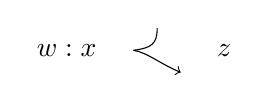
\begin{tikzpicture}[baseline=(x.base)]
\node (x) at (0,0) {$w:x$};
\node at (2,0) {$z$};
\draw (1.15,.28) .. controls (1.15,.08) and (1.08,.03) .. (.85,0);
\draw[->] (.85,0) .. controls (1.03,-.03) and (1.2,-.18) .. (1.45,-.28);
\end{tikzpicture}}.
De plus, on a
\[
x\not\prec x\qquad\left(\text{car }\operatorname{Im}(\Sigma_1\overset{(p_1;\uline{b})}{\relbar\joinrel\relbar}\Sigma\times\Sigma)\cap\text{diag}=\varnothing\right)
\]
% The final = empty-set and the end of the parenthesis continue below at the right.
donc la relation $x\prec y$ est la relation
d'inégalité stricte associée à une relation
d'ordre sur $\Sigma$. On récupère $\Sigma^{\unsure{<|*}}(1)$ comme
le graphe de la relation d'ordre stricte,
$\Sigma^{<}(2)$ comme les drapeaux $x\prec y\prec z$ de
longueur $2$ dans \illegible{1} $\Sigma$, et les applications
% A separate small curved upright is raised in the gap after dans, before Sigma;
% its value is unassigned. It is preserved above as an unread fragment.
% Pale lower-left foliation, apparently another hand; no top authorial number is visible.
\margin{59}

\scanpage{62}
b) L'application $\Sigma^{<}(2)\xrightarrow{(p_1\circ s',\unsure{p_1b'|p_1\circ b'})}\Sigma\times\Sigma$
se factorise par $\Sigma^{<}(1)\lhook\joinrel\xrightarrow{(p_1,\uline{b})}\Sigma\times\Sigma$
en un morphisme
\[
p_2:\Sigma^{<}(2)-\Sigma^{<}(1)
\]
qui rende le carré
\diagram{\begin{tikzcd}[
  column sep={40mm,between origins},
  row sep={16.5mm,between origins},
  nodes={shape=rectangle,anchor=center,inner sep=0pt,outer sep=0pt},
  arrows={line width=.4pt,>=stealth,shorten <=0pt,shorten >=0pt},
  execute at end picture={
    \begin{scope}[shift={(s62a.center)},x=1cm,y=1cm,line width=.4pt]
    % UH1--UH4: the four separate upper hook fragments.
    \draw[line width=.4pt] (1.12,.22)--(1.06,.20);
    \draw[line width=.4pt] (.98,.15)--(.94,.12);
    \draw[line width=.4pt] (.94,.05)--(.98,.01);
    \draw[line width=.4pt] (1.05,-.02)--(1.12,-.02);
    % LH1--LH2: the two separate lower hook fragments.
    \draw (2.18,-1.40) .. controls (2.10,-1.39) and (2.08,-1.43) .. (2.06,-1.47);
    \draw[line width=.4pt] (2.07,-1.54)--(2.09,-1.58);
    % LS1--LS2: the lower shaft retains the gap from x=2.55 to x=2.62.
    \draw (2.21,-1.62)--(2.55,-1.62);
    \draw (2.62,-1.62)--(3.28,-1.62);
    % LR: the second, lower trace of the elongated open loop.
    \draw (3.24,-1.62) .. controls (3.58,-1.77) and (4.00,-1.73) .. (4.18,-1.62);
    % All four labels keep the accepted positions and underline scopes.
    \node at (2.35,.22) {$\uline{b}'$};
    \node at (.93,-.68) {$p_2$};
    \node at (4.75,-.65) {$p_1$};
    \node at (2.75,-1.32) {$\uline{b}$};
    \end{scope}
  }
]
|[alias=s62a]| \Sigma^{\unsure{<|*}}(2)
  \arrow[r,no head,to path={
    ([xshift=11.7mm,yshift=-.4mm]s62a.center)--
    ([xshift=34.5mm,yshift=-.4mm]s62a.center)
    .. controls ([xshift=35mm,yshift=-.4mm]s62a.center)
    and ([xshift=35mm,yshift=-.1mm]s62a.center)
    .. ([xshift=34.8mm,yshift=.5mm]s62a.center)
  }]
  \arrow[d,->,to path={
    ([xshift=2.5mm,yshift=-4.5mm]s62a.center)--
    ([xshift=10.3mm,yshift=-12.9mm]s62a.center)
  }]
&
|[alias=s62b]| \Sigma^{<}(1)
  \arrow[d,->,to path={
    ([xshift=42mm,yshift=-3.8mm]s62a.center)--
    ([xshift=48.7mm,yshift=-12.5mm]s62a.center)
  }]
\\
|[alias=s62c,xshift=15mm]| \Sigma^{<}(1)
  \arrow[r,->,to path={
    ([xshift=32.8mm,yshift=-16.2mm]s62a.center)
    .. controls ([xshift=36.5mm,yshift=-15.9mm]s62a.center)
    and ([xshift=40.2mm,yshift=-16mm]s62a.center)
    .. ([xshift=43.2mm,yshift=-16.2mm]s62a.center)
  }]
&
|[alias=s62d,xshift=10mm]| \Sigma
\end{tikzcd}}
\uline{Cartésien}, et $p_1:\Sigma^{<}(1)-\Sigma$ étant transversal
à \deleted{\unsure{l'imm}}ersion-but $\uline{b}:\Sigma^{\unsure{<|*}}(1)-\Sigma$.
\margin{\uline{NB} (Si $\Sigma$ est séparé, donc $\Sigma\times\Sigma$ séparé
sur $\Sigma$, et $\Sigma^{<}(1)\overset{\uline{b}}{-}\Sigma$
propre, il en résulte
que $\Sigma^{<}(1)-\Sigma\times\Sigma$ est
propre donc un plongement
\uline{fermé}.}
\margin{cette condition de transversalité est
peut être conséquence des autres .-}

De façon équivalente, une telle structure
est donnée par un espace topologique \inserted{séparé} $\Sigma$,
muni d'une relation d'ordre $x\preceq y$
\deleted{dont le graphe est}\inserted{satisfaisant les conditions suivantes}

% Two unassigned dark points beside the first cancelled a) line.
\margin{\figure{\begin{tikzpicture}[x=1mm,y=1mm]
\fill (0,0) circle (.16mm);
\fill (.5,-.8) circle (.16mm);
\end{tikzpicture}}}
\deleted{a) le graphe \deleted{$\unsure{\Sigma^{<}(1)|\Sigma^{*}(1)}$} $\Sigma(1)$ de cette relation est
fermé dans $\Sigma\times\Sigma$, et $\Sigma(1)\overset{\uline{b}}{-}\Sigma$ est
une immersion\unsure{.}
\deleted{$\unsure{\Sigma}$}
b) Si $\Sigma^{*}(1)$ est le graphe de la
relation d'ordre \inserted{stricte}, $\Sigma^{*}(1)\xrightarrow{\uline{b}}\Sigma$ est une
immersion \inserted{bordante} propre \deleted{\unsure{(donc la partie de}}
a) Si $x\in\Sigma$, $\Sigma_{<x}$ \inserted{$(=\Sigma^{\unsure{<|*}}(1)_{\unsure{x}})$}\unsure{,}
\unsure{\deleted{\unsure{est} \unsure{un|une}}|\unsure{est} \unsure{un|une}}
\unsure{ens|est} (fini) \uline{tot}$ {}^t$. \uline{ordonné}.
}
\margin{\handwritten{61}}

\scanpage{63}
\mspage{27}
\deleted{c) Si $(z_\alpha)_{\alpha\in I}$ est l'ens des éléments de
$\Sigma_{<x}=\uline{b}^{-1}(\{x\})$ (où $\uline{b}:\Sigma^{\unsure{<|*}}(1)\longrightarrow\Sigma$), les
\unsure{les};}

a) Pour \unsure{tt|$\forall$} $x\in\Sigma$, l'ens $\Sigma_{<x}$ \deleted{(fini) \unsure{est}}\inserted{est tot${}^t$}
\deleted{$\simeq\uline{b}^{-1}(\{x\}$} ordonné

b) Si $\Sigma^{\unsure{*|<}}(1)$ est le graphe de la relation
$x<y$, et $\uline{s},\uline{b}:\Sigma^{<}(1)\unsure{\rightrightarrows|=}\Sigma$ sont les applications
source et but, \deleted{\illegible{1}} l'application $\uline{b}$ est une immer-
sion \deleted{\uline{\unsure{bordante}}} \uline{propre} (donc les $\Sigma_{<x}\unsure{\ne|=}\uline{b}^{-1}(\{x\})$
sont finis)

c) Si $(z_\alpha)_{\alpha\in I}$ sont les éléments de $\Sigma_{<x}=b^{-1}(\{x\})$,
alors \inserted{la famille} \unsure{des|les} \unsure{g}ermes \inserted{en $x$} de sous-espaces \deleted{\unsure{bordants}}\inserted{de $\Sigma$}
images par $\uline{b}$ des \inserted{germes} $(\Sigma^{<}(1),z_\alpha)$, est \inserted{une famille}
\deleted{\unsure{transversaux}}\inserted{transversale}
de sous-espaces \uline{bordants}.

d) $\uline{\unsure{b|s|p_1}}:\Sigma^{<}(1)\longrightarrow\Sigma^*$ est \uline{transversal} p.r. à l'immersion
bordante $\uline{b}:\Sigma^{<}(1)\mathrel{-}\Sigma^{\unsure{*}}$
\deleted{\unsure{la diag.}}
\margin{ou sous forme d'une \unsure{récollection|récollement}
pour les $z_\alpha\in\Sigma^{<}(1)$ au dessus d'un même
$x\in\Sigma^*$\ldots}

$1^{\circ})$ Cas équisingulier : $\uline{s}:\Sigma^{<}(1)\mathrel{-}\Sigma$ fibrant \inserted{(propre)}

$2^{\circ})$ Cas non singulier : $\unsure{\Sigma}$ est une variété à bord,
dont le bord est $\uline{b}(\Sigma^{*}(1))$:

$3^{\circ})$ Cas \unsure{équisingulier|équi-singulier}-non-singulier : $\uline{s}:\Sigma^{<}(1)\mathrel{-}\Sigma$ est
fibrant \inserted{propre}, à fibres des variétés à bord, et le
fibré des bords est l'image de $\Sigma^{*}(2)$ par
le morphisme $\Sigma^{*}(2)\xrightarrow{\uline{s'}}\Sigma^{\unsure{*|<}}(1)$ \deleted{\unsure{avec}}\inserted{donné}
par $(x\prec y\prec z)\longrightarrow(x\prec z)$.
\margin{c'est sans doute conséquence de la conjonction des deux conditions $1^{\circ}),2^{\circ})$}
\margin{62}

\scanpage{64}
Les morphismes les plus importants dans la
situation apparaissent dans le diagramme
% The curved leader attaches hexagonal immediately before the live suivant.
\inserted{hexagonal} suivant
\diagram{\begin{tikzcd}[column sep=9mm,row sep=13mm,arrows={line width=.6pt},execute at end picture={
% Upper b: four separate hook components, with unequal lengths.
\draw[line width=.7pt,line cap=round] ([xshift=7.1pt,yshift=6.0pt]s64upper.east) -- ([xshift=8.6pt,yshift=6.6pt]s64upper.east);
\draw[line width=.6pt,line cap=round] ([xshift=5.3pt,yshift=4.6pt]s64upper.east) -- ([xshift=4.6pt,yshift=3.6pt]s64upper.east);
\draw[line width=.6pt,line cap=round] ([xshift=4.3pt,yshift=2.5pt]s64upper.east) .. controls +(0pt,-1.5pt) and +(-1pt,0pt) .. ([xshift=5.4pt,yshift=.8pt]s64upper.east);
\draw[line width=.6pt,line cap=round] ([xshift=6.4pt,yshift=.5pt]s64upper.east) .. controls +(.5pt,.2pt) and +(-.5pt,0pt) .. ([xshift=7.6pt,yshift=.8pt]s64upper.east);
% Central b-prime: four components; the second one is visibly faint.
\draw[line width=.6pt,line cap=round] ([xshift=7.2pt,yshift=6.2pt]s64centre.east) -- ([xshift=8.2pt,yshift=6.8pt]s64centre.east);
\draw[line width=.4pt,black!45,line cap=round] ([xshift=5.9pt,yshift=5.3pt]s64centre.east) -- ([xshift=5.2pt,yshift=4.5pt]s64centre.east);
\draw[line width=.6pt,line cap=round] ([xshift=4.4pt,yshift=3.3pt]s64centre.east) .. controls +(0pt,-1.5pt) and +(-.2pt,.5pt) .. ([xshift=4.4pt,yshift=1.6pt]s64centre.east);
\draw[line width=.6pt,line cap=round] ([xshift=5.3pt,yshift=1.0pt]s64centre.east) -- ([xshift=7.1pt,yshift=.6pt]s64centre.east);
% Upper-right b: three detached pieces at the source.
\draw[line width=.6pt,line cap=round] ([xshift=-8.7pt,yshift=4.8pt]s64right.north west) .. controls +(-.7pt,.9pt) and +(0pt,-.5pt) .. ([xshift=-9.1pt,yshift=6.0pt]s64right.north west);
\draw[line width=.6pt,line cap=round] ([xshift=-8.0pt,yshift=3.8pt]s64right.north west) -- ([xshift=-6.7pt,yshift=3.1pt]s64right.north west);
\draw[line width=.6pt,line cap=round] ([xshift=-5.6pt,yshift=3.0pt]s64right.north west) .. controls +(.6pt,0pt) and +(-.4pt,-.4pt) .. ([xshift=-4.5pt,yshift=3.5pt]s64right.north west);
% Lower b: one detached upper curl, and one lower bend joined to the shaft.
\draw[line width=.7pt,line cap=round] ([xshift=4.7pt,yshift=4.1pt]s64lower.east) .. controls +(0pt,1pt) and +(-.8pt,.4pt) .. ([xshift=6.4pt,yshift=5.3pt]s64lower.east);
\draw[line width=.6pt,line cap=round] ([xshift=4.0pt,yshift=2.4pt]s64lower.east) .. controls +(-.2pt,-2.6pt) and +(-2pt,0pt) .. ([xshift=7pt]s64lower.east);
% s-prime: two unequal visible shafts merge at one head.  Its source curl
% comprises a long U-like part and a separate right arc, with a pen gap.
\draw[->,line width=.85pt,line cap=round] ([xshift=-2.5pt,yshift=8.0pt]s64centre.north west) -- ([yshift=-2pt]s64upper.south east);
\draw[line width=.5pt,line cap=round] ([xshift=.8pt,yshift=9.1pt]s64centre.north west) .. controls +(-3pt,4pt) and +(4pt,-3pt) .. ([yshift=-2pt]s64upper.south east);
\draw[line width=.7pt,line cap=round] ([xshift=-10pt,yshift=7pt]s64centre.north west) .. controls +(0pt,-3pt) and +(-2pt,0pt) .. ([xshift=-3.5pt,yshift=4.5pt]s64centre.north west) .. controls +(1.5pt,0pt) and +(0pt,-1.3pt) .. ([xshift=-2pt,yshift=6.3pt]s64centre.north west);
\draw[line width=.6pt,line cap=round] ([xshift=-.8pt,yshift=5.1pt]s64centre.north west) .. controls +(2.1pt,.6pt) and +(1pt,-1pt) .. ([xshift=1.2pt,yshift=8.0pt]s64centre.north west);
\node[anchor=east] at ([xshift=-18mm,yshift=3pt]s64left.west) {$(40)$};
\node[anchor=west] at ([xshift=34mm,yshift=-3mm]s64bottom.east) {,};
}]
&|[alias=s64upper]|\Sigma^{\unsure{<|*}}(1)\arrow[rr,"\uline{b}",start anchor=east,shorten <=9pt]\arrow[dl,"\uline{s}"']&&|[alias=s64top]|\Sigma&\\
|[alias=s64left]|\Sigma&&|[alias=s64centre]|\Sigma^{*}(2)\arrow[ul,phantom,"\uline{s'}"']\arrow[rr,"\uline{b}'",start anchor=east,shorten <=9pt]\arrow[dl,"\uline{p}"']\arrow[ur,phantom,"\text{cart}" description]\arrow[dr,phantom,"\text{cart}" description]&&|[alias=s64right]|\Sigma^{\unsure{<|*}}(1)\arrow[ul,"\uline{b}"',start anchor=north west,shorten <=7pt]\arrow[dl,"\uline{s}"]\\
&|[alias=s64lower]|\Sigma^{\unsure{<|*}}(1)\arrow[ul,"\uline{s}"']\arrow[rr,"\uline{b}",start anchor=east,shorten <=7pt]&&|[alias=s64bottom]|\Sigma&
\end{tikzcd}}

où les flèches marquées \diagram{\begin{tikzcd}[column sep=large,arrows={line width=.6pt},execute at end picture={
% Four disconnected marks: an upper slant, then three short dot-like pieces.
\draw[line width=.7pt,line cap=round] ([xshift=6.3pt,yshift=6.1pt]s64legend.east) -- ([xshift=8pt,yshift=6.8pt]s64legend.east);
\fill ([xshift=5.1pt,yshift=4.8pt]s64legend.east) circle[radius=.48pt];
\fill ([xshift=5.3pt,yshift=3.1pt]s64legend.east) circle[radius=.48pt];
\fill ([xshift=6pt,yshift=1.7pt]s64legend.east) circle[radius=.43pt];}]
|[alias=s64legend]|{}\arrow[r,start anchor=east,shorten <=8pt]&{}
\end{tikzcd}} (en fait,
$\uline{b},\deleted{\unsure{p_2}},\uline{b'},\uline{s'}$) sont des immersions bordantes \inserted{propres},
% propres is above bordantes; its surrounding curve continues into the
% insertion leader, ending after bordantes before the separate comma.
et les flèches marquées $\longrightarrow$ (en fait,
$\uline{s}$ et $\uline{p}$) sont (dans le cas équisingulier)
fibrantes et propres \unsure{\}} (\unsure{voire|voir}, de plus : fibres
des variétés à bord, dont le bord est
dans le cas de $\unsure{\uline{s}|\uline{s'}}:\Sigma^{\unsure{<|*}}(1)\longrightarrow\Sigma$, l'image
% A short dark raised stroke above this s may be a pen-start or a prime;
% both readings are retained.  No identification with the later s-prime is imposed.
de $\Sigma^{\unsure{<|*}}(2)\overset{\uline{s'}}{-}\Sigma^{*}(1)$
% The initial curve before i.e. continues below the insertion and into its
% long leader.  It is not separately repeated as a literal parenthesis.
\inserted{i.e. l'ens des $(x\prec y)$ tels que $y$ \uline{ne soit pas} successeur de $x$}).
% The insertion is above this map; successeur de x wraps at its right end.
% The following note is oblique in the left margin beside the fibre/boundary passage.
\margin{donc, dans le cas de $\uline{p}:\Sigma^{\unsure{<|*}}(2)\mathrel{\unsure{-|\longrightarrow}}\Sigma^{\unsure{*|<}}(1)$,
le fibré des bords est l'image de $\Sigma^{\unsure{<|*}}(3)$}
On fera attention
que les applications fibrantes $\uline{s},\uline{p}$ n'ont \deleted{\unsure{rien}}\inserted{rien}
de surjectif --- l'image de $\unsure{\uline{s}|s}$ est formé des $x\in\Sigma$
qui \uline{ne sont pas maximaux}, celle de $p$ est formé
des $(x\prec y)$ tels que $y$ ne soit pas maximal.
% Pale bottom-left foliation, another hand; no authorial page number at the head.
\margin{63}

\scanpage{65}
\mspage{28}
\uline{12} Récapitulation (des données de déploiement,
relatif à un ens ordonné $I$, fini disons\ldots)

\[
\left\{\begin{aligned}
\text{a) }&\text{Espaces }\Sigma_i\quad(i\in I)\\
\text{b) }&\text{Espaces }\Sigma_{i,j}\quad(i<j,\ i,j\in I)\\
\text{c) }&\text{Applications }\Sigma_{i,j}\xrightarrow{s_{ij}}\Sigma_i,\quad
\Sigma_{ij}\xrightarrow{b_{ij}}\Sigma_j
\end{aligned}\right.
\]
\margin{C'est la structure envisagée dans le Scholie (p. $26/27$)
plus une application continue strictement croissante
$\Sigma\overset{\varphi}{\unsure{-|\longrightarrow}}I$, telle que
$\forall x\in\Sigma$, $\varphi|\Sigma_{<x}$ soit injective
(\uline{donc} la relation d'ordre de
\inserted{\unsure{(pour $i$ ?)}} $\Sigma_{<x}$
soit induite par celle de $I_{<i}$)}

Conditions

a) $\Sigma_{ij}\longrightarrow\Sigma_j$
\deleted{\unsure{immersion}}\inserted{plongement} fermé
\deleted{bordant}
\inserted{[On identifie $\Sigma_{ij}$ à un ss-espace fermé de
$\Sigma_j$ par $b_{ij}$]}

b) $\Sigma_{i,k}\cap\Sigma_{j,k}=\varnothing$ si $i,j$,
\deleted{$\unsure{\exists}$} non comparables
\deleted{\unsure{(on suppose|(on supp}}
\unsure{\inserted{\deleted{\unsure{($i<j$)}}}|\deleted{\unsure{($i<j$)}}}
(NB $i,j<k$)
\margin{\uline{NB} La condition \uline{b}) équivaut à celle
que dans l'ens ordonné $\Sigma=\coprod\Sigma_i$, les ensembles
$\Sigma_{<x}$ sont tot$ {}^t$ ordonnés}

c) Pour $\unsure{\deleted{\unsure{i}}|\unsure{i}}\ i<j<k$ posons
\[
\Sigma_{ijk}=\Sigma_{ik}\cap\Sigma_{jk}
\uline{\subset\unsure{\Sigma_k}}.
\]
On a alors \inserted{dans $\Sigma_{jk}$ :}
\deleted{$\unsure{\Sigma_{jk}}$}
\figure{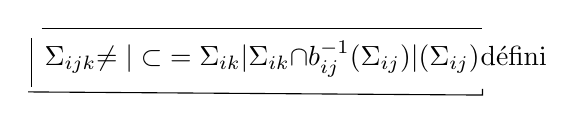
\begin{tikzpicture}[baseline=(eq.base)]
\node[anchor=base west,inner sep=0pt] (eq) at (0,0)
{$\Sigma_{ijk}\deleted{\unsure{\ne|\subset}}=
\deleted{\unsure{\Sigma_{ik}|\Sigma_{ik}\cap}}
b_{ij}^{-1}\unsure{(\Sigma_{ij})|\deleted{(\Sigma_{ij})}}$};
\node[anchor=base west,inner sep=0pt] at (eq.base east)
{\deleted{\unsure{défini}}};
\draw ([xshift=-.03cm,yshift=.16cm]eq.north west)
-- ([xshift=.03cm,yshift=.16cm]eq.north east);
\draw ([xshift=-.16cm,yshift=.03cm]eq.north west)
-- ([xshift=-.16cm,yshift=-.12cm]eq.south west);
\draw ([xshift=-.20cm,yshift=-.18cm]eq.south west)
-- ([xshift=.03cm,yshift=-.22cm]eq.south east)
-- ([xshift=.03cm,yshift=-.14cm]eq.south east);
\end{tikzpicture}}
\deleted{\unsure{une}}

On a donc, pour $i<j<k$, un diagramme
commutatif hexagonal
\diagram{\begin{tikzcd}[
  /tikz/x=1.15cm,/tikz/y=1.15cm,
  column sep={1.15cm,between origins},
  row sep={1.725cm,between origins},
  cells={nodes={anchor=center}},
  /tikz/execute at end picture={
    \node[anchor=center] at ([xshift=-1.725cm,yshift=0.0575cm]scan065I.center) {(41)};
    \node[anchor=center] at ([xshift=0.736cm,yshift=1.2075cm]scan065I.center) {$s_{ik}$};
    \node[anchor=center] at ([xshift=3.3465cm,yshift=2.2425cm]scan065I.center) {$b_{ik}$};
    \node[anchor=center] at ([xshift=6.371cm,yshift=1.219cm]scan065I.center) {$b_{jk}$};
    \node[anchor=center] at ([xshift=0.7245cm,yshift=-1.2305cm]scan065I.center) {$s_{ij}$};
    \node[anchor=center] at ([xshift=3.4155cm,yshift=-2.2655cm]scan065I.center) {$b_{ij}$};
    \node[anchor=center] at ([xshift=5.9915cm,yshift=-0.966cm]scan065I.center) {$s_{jk}$};
    \node[anchor=center] at ([xshift=4.1055cm,yshift=0.989cm]scan065I.center) {cart};
    \node[anchor=center] at ([xshift=4.186cm,yshift=-0.8165cm]scan065I.center) {cart};
    % The two detached points retain their accepted radii and remain unassigned.
    \fill ([xshift=2.691cm,yshift=-2.2655cm]scan065I.center) circle (.012);
    \fill ([xshift=2.7485cm,yshift=-2.1965cm]scan065I.center) circle (.012);
  }
]
 & |[alias=scan065IK,xshift=0.805cm]| \Sigma_{ik} & & |[alias=scan065K,xshift=1.38cm]| \Sigma_k & \\
|[alias=scan065I,yshift=-0.115cm]| \Sigma_i & & |[alias=scan065IJK,xshift=0.805cm]| \Sigma_{ijk} & & |[alias=scan065JK,xshift=1.955cm]| \Sigma_{jk} \\
 & |[alias=scan065IJ,xshift=0.805cm]| \unsure{\Sigma}_{ij} & & |[alias=scan065J,xshift=1.38cm]| \Sigma_j &
% E1: IK -> I; accepted path coordinates, translated with scan065I.
\arrow[from=1-2,to=2-1,
  /tikz/arrows=->,/tikz/>=to,/tikz/line width=.4pt,
  /tikz/shorten >=0pt,/tikz/shorten <=0pt,
  to path={
    ([xshift=1.426cm,yshift=1.4145cm]scan065I.center)--([xshift=0.4945cm,yshift=0.4945cm]scan065I.center)
    \tikztonodes
  }]
% E2: IK -> K; accepted path coordinates, translated with scan065I.
\arrow[from=1-2,to=1-4,
  /tikz/arrows=->,/tikz/>=to,/tikz/line width=.4pt,
  /tikz/shorten >=0pt,/tikz/shorten <=0pt,
  to path={
    ([xshift=2.645cm,yshift=2.0125cm]scan065I.center)
    ..controls ([xshift=2.3575cm,yshift=1.8975cm]scan065I.center) and ([xshift=2.369cm,yshift=1.6905cm]scan065I.center)..([xshift=2.6565cm,yshift=1.6905cm]scan065I.center)
    --([xshift=4.048cm,yshift=1.6905cm]scan065I.center)
    \tikztonodes
  }]
% E3: JK -> K; accepted path coordinates, translated with scan065I.
\arrow[from=2-5,to=1-4,
  /tikz/arrows=->,/tikz/>=to,/tikz/line width=.4pt,
  /tikz/shorten >=0pt,/tikz/shorten <=0pt,
  to path={
    ([xshift=5.865cm,yshift=0.7475cm]scan065I.center)
    ..controls ([xshift=6.325cm,yshift=0.5175cm]scan065I.center) and ([xshift=6.325cm,yshift=0.943cm]scan065I.center)..([xshift=5.4855cm,yshift=1.4605cm]scan065I.center)
    \tikztonodes
  }]
% E4: IJK -> IK; accepted path coordinates, translated with scan065I.
\arrow[from=2-3,to=1-2,
  /tikz/arrows=->,/tikz/>=to,/tikz/line width=.4pt,
  /tikz/shorten >=0pt,/tikz/shorten <=0pt,
  to path={
    ([xshift=2.645cm,yshift=0.782cm]scan065I.center)
    ..controls ([xshift=3.0475cm,yshift=0.552cm]scan065I.center) and ([xshift=3.036cm,yshift=0.943cm]scan065I.center)..([xshift=2.3805cm,yshift=1.38cm]scan065I.center)
    \tikztonodes
  }]
% E5: IJK -> JK; accepted path coordinates, translated with scan065I.
\arrow[from=2-3,to=2-5,
  /tikz/arrows=->,/tikz/>=to,/tikz/line width=.4pt,
  /tikz/shorten >=0pt,/tikz/shorten <=0pt,
  to path={
    ([xshift=3.772cm,yshift=0.322cm]scan065I.center)
    ..controls ([xshift=3.4845cm,yshift=0.1955cm]scan065I.center) and ([xshift=3.496cm,yshift=0.023cm]scan065I.center)..([xshift=3.7605cm,yshift=0.023cm]scan065I.center)
    --([xshift=5.7155cm,yshift=0.023cm]scan065I.center)
    \tikztonodes
  }]
% E6: IJK -> IJ; accepted path coordinates, translated with scan065I.
\arrow[from=2-3,to=3-2,
  /tikz/arrows=->,/tikz/>=to,/tikz/line width=.4pt,
  /tikz/shorten >=0pt,/tikz/shorten <=0pt,
  to path={
    ([xshift=2.714cm,yshift=-0.322cm]scan065I.center)--([xshift=2.277cm,yshift=-1.081cm]scan065I.center)
    \tikztonodes
  }]
% E7: IJ -> I; accepted path coordinates, translated with scan065I.
\arrow[from=3-2,to=2-1,
  /tikz/arrows=->,/tikz/>=to,/tikz/line width=.4pt,
  /tikz/shorten >=0pt,/tikz/shorten <=0pt,
  to path={
    ([xshift=1.426cm,yshift=-1.288cm]scan065I.center)--([xshift=0.4945cm,yshift=-0.4945cm]scan065I.center)
    \tikztonodes
  }]
% E8: IJ -> J; accepted path coordinates, translated with scan065I.
\arrow[from=3-2,to=3-4,
  /tikz/arrows=->,/tikz/>=to,/tikz/line width=.4pt,
  /tikz/shorten >=0pt,/tikz/shorten <=0pt,
  to path={
    ([xshift=2.76cm,yshift=-1.4145cm]scan065I.center)
    ..controls ([xshift=2.4495cm,yshift=-1.564cm]scan065I.center) and ([xshift=2.4495cm,yshift=-1.7365cm]scan065I.center)..([xshift=2.7485cm,yshift=-1.7365cm]scan065I.center)
    --([xshift=4.0595cm,yshift=-1.7365cm]scan065I.center)
    \tikztonodes
  }]
% E9: JK -> J; accepted path coordinates, translated with scan065I.
\arrow[from=2-5,to=3-4,
  /tikz/arrows=->,/tikz/>=to,/tikz/line width=.4pt,
  /tikz/shorten >=0pt,/tikz/shorten <=0pt,
  to path={
    ([xshift=5.957cm,yshift=-0.3335cm]scan065I.center)--([xshift=5.3475cm,yshift=-1.288cm]scan065I.center)
    \tikztonodes
  }]
\end{tikzcd}}

où les flèches $\lhook\joinrel\relbar\joinrel\relbar$ sont des inclusions
fermees \inserted{cf plus bas} (bordantes), et les flèches
\(\mathrel{\begin{tikzpicture}[baseline=-.35ex,x=1cm,y=1cm]
\draw[->] (0,0)--(1.2,0);
\fill (.45,.55) circle (.016);
\end{tikzpicture}}\)
sont des applications qui seront fibrantes et propres
dans le cas équisingulier.
\margin{\handwritten{64}}

\scanpage{66}
d) \deleted{\unsure{a}} Les $\Sigma_j\hookrightarrow\Sigma_{ji}$ sont bordants, et si
$x\in\Sigma_i$, \deleted{les} \unsure{dans|donc} les $\Sigma_{ji}\ni x$ (\deleted{pour $j<i$}\inserted{indices}
\deleted{\unsure{tels que}}\deleted{$\Sigma$}\inserted{par l'ens}. $I_{<i,x}\overset{\mathrm{def}}{=}\{j\in I\mid j<i,\ \Sigma_{ji}\ni x\}$,
qui est totalement ordonné par b) sont
des sous-espaces-bords transversaux en $x$
--- i.e. les $\Sigma_{ji}$ $(j\in I_{<i})$ sont des
sous-espaces bords de $\Sigma_i$ \unsure{mutuell\({}^t\)}
transversaux.

e) $\Sigma_{\unsure{i|j}j}\xrightarrow{s_{ij}}\Sigma_i$ est transversal p.r. au système \unsure{trans}-
versal des morphismes bordants
$b_{\unsure{ik|ki}}:\Sigma_{\unsure{k}i}\longrightarrow\Sigma_i$

Si on pose
\[
\Sigma=\coprod_{i\in I}\Sigma_i
\]
\[
\Sigma^{<}(1)=\coprod_{\substack{i,j\in I\\i<j}}\Sigma_{ij}
\]
et $\uline{s},\uline{b}:\Sigma^{<}(1)\mathrel{-}\Sigma$ induits par les
$s_{ij},b_{ij}$, alors les conditions a) b) c)
signifient que $(\uline{s},\uline{b}):\Sigma^{<}(1)\longrightarrow\Sigma\unsure{\times|<}\Sigma$ est
inj. et a comme \deleted{\unsure{graphe}}\inserted{image} le graphe d'une
relation d'ordre \unsure{stricte|strict}, avec $\uline{b}:\Sigma^{<}(1)\longrightarrow\Sigma$
\inserted{immersion} propre, \deleted{et} que l'application \inserted{continue évidente} $\varphi:\Sigma^{\unsure{*}}\unsure{\ell|\deleted{\ell}}\longrightarrow\unsure{\deleted{\Sigma}I|I}$
est strict\({}^t\) croissante, et que pour \unsure{tt|$\forall$} $x\in\Sigma$,
l'application induite $\varphi:\Sigma_{<x}\mathrel{-}I_{<i}$ $(i=\varphi(x))$ est
injective, enfin que $\Sigma_{<x}$ est \unsure{tot.|tt.} ordonné.
\margin{65}

\scanpage{67}
\mspage{29}
Enfin, la condition d) signifie que cette structure
\inserted{d'espace top. ordonné}
% The initial d is reworked but live.  The parenthesis-like curve before
% satisfait belongs to the continuous insertion leader beneath ordonné.
satisfait la condition c) du Scholie (p. $27$).

\uline{Cas équisingulier} : les $s_{ij}$ sont fibrants propres

\uline{Cas non singulier} : les $\Sigma_i$ sont des variétés
% The dotted i in this first Sigma subscript is locally reworked;
% no independently recoverable underlying letter is supplied.
topologiques\unsure{,|;} le bord de $\Sigma_i$ est la réunion
% The comma is clear; a tiny separate point above it has uncertain attachment
% and provenance, so the semicolon alternative remains local and explicit.
des $\Sigma_{ji}$ pour $j<i$ \deleted{(NB il suffit
de prendre pour $j$}
\margin{On voudra que de $=$ les $\Sigma_{ij}$ soient des variétés à bord, que le
bord soit la réunion des $\Sigma_{kij}$ et $\Sigma_{ikj}$ --- mais
c'est sans doute une conséquence de la condition précédente..-}

\uline{Cas} \uline{équisingulier}-\uline{non singulier}
$s_{ij}:\unsure{\Sigma_{ik}|\Sigma_{i\deleted{j}k}|\Sigma_{ij}}\longrightarrow\Sigma_j$ est
% The source's upper k-like form lies over a long hooked lower trace.
% Alternatives retain both the literal ik and an uncertain overwritten j layer.
une fibration propre, à fibres des variétés
\margin{\figure{\begin{tikzpicture}[x=1mm,y=1mm]
% Unassigned thin broken stroke at the right paper edge; provenance uncertain.
\draw[black!55,line width=.2pt] (0,0)--(.8,.15);
\draw[line width=.23pt] (1.1,.18)--(2.3,.3);
\draw[line width=.23pt] (2.6,.32)--(4.6,.5);
\draw[line width=.23pt] (4.9,.53)--(6.9,.72);
\draw[line width=.23pt] (7.1,.74)--(9.5,.95);
\end{tikzpicture}}}
à bord, le fibré des bords est réunion
des $\Sigma_{ijk}$ pour $i<\deleted{\unsure{j}}\inserted{j}<k$.
% The cancelled central glyph lies below/through the higher rewritten j;
% the older glyph's reading as j is tentative, not a recovered certainty.

13. \uline{Une digression} Revenons au cas de
$\Sigma,\Sigma^{\unsure{*|<}}(1)\subset\Sigma\times\unsure{\Sigma|\overline{\Sigma}}$, sans donnée de $I$. Plus
% The last Sigma has a detached upper bar.  The four-stroke construction
% favours a pen-lift within Sigma; an additional overline remains an alternative.
généralement, considérons une \uline{catégorie topologique}
\diagram{\begin{tikzcd}[column sep=5mm,arrows={line width=.6pt},execute at end picture={
% The lower connector ends in the observed dense short upright/stub.
\fill ([xshift=-2.8pt,yshift=-1.35pt]s67pairtarget.west) --
([xshift=-1.4pt,yshift=-2.2pt]s67pairtarget.west) --
([xshift=-1.8pt,yshift=-3.5pt]s67pairtarget.west) --
([xshift=-3.0pt,yshift=-3.2pt]s67pairtarget.west) -- cycle;
}]
{\uline{\Sigma}=(\Sigma_{(0)}=\operatorname{Ob}(\uline{\Sigma}),\quad\Sigma_{(1)}=\operatorname{Fl}(\uline{\Sigma}),}
& \Sigma_{(1)}\arrow[r,shift left=2.5,"\uline{s}"]\arrow[r,shift right=2.5,dash,"\uline{b}"',end anchor=west,shorten >=2pt]
& |[alias=s67pairtarget]|\Sigma_{(0)},
\end{tikzcd}}
\diagram{\begin{tikzcd}[column sep=10mm,arrows={line width=.6pt},execute at end picture={
% Definition connector: the upper bar is shorter and detached from the
% lower shaft's single right head.  Two dark points below it remain unassigned.
\draw[->,line width=.75pt,line cap=round] ([xshift=2pt,yshift=-1pt]s67product.east) -- ([xshift=-2pt,yshift=-1pt]s67two.west);
\draw[line width=.55pt,line cap=round] ([xshift=2pt,yshift=3pt]s67product.east) -- ([xshift=-5pt,yshift=3pt]s67two.west);
\fill ([xshift=-7pt,yshift=-5pt]s67two.west) circle[radius=.27pt];
\fill ([xshift=-7.7pt,yshift=-6.5pt]s67two.west) circle[radius=.23pt];
}]
|[alias=s67product]|(\Sigma_{(1)},b)\times_{\Sigma_{(0)}}(\Sigma_{(\unsure{1})},s)\arrow[r,phantom,"\text{déf}"]
& |[alias=s67two]|\Sigma_{(2)}\arrow[r,"\unsure{\text{cpl.}|\text{compl.}}","\substack{\text{comp.}\\\text{des flèches}}"']
& \Sigma_{(1)}
\end{tikzcd}}
), et supposons
que $\uline{s}:\Sigma_{(1)}\unsure{\longrightarrow|-}\Sigma_{(0)}$ soit \uline{fibrant}. Je dis
% The short filled terminal of this shaft is pointed but densely inked.
qu'alors $\pi_0(\Sigma_{(0)})=\unsure{I_{(\deleted{\unsure{0}}\uline{\Sigma})}|I(\deleted{\unsure{0}}\uline{\Sigma})|I_{(0)}}$ est \uline{un ens. }\inserted{pré\deleted{\unsure{filtré}}}\uline{ordonné},
% The I expression has a compact, lowered-looking parenthesised overwork:
% a Sigma-like form and zero-like residual loops.  Both layer and vertical
% placement remain uncertain in the explicit alternatives.
% Live pré lies to the left of the crossed interlinear filtré candidate;
% the common curved leader enters before the live baseline ordonné.
% The continuous baseline underline spans un ens. and ordonné.
en prenant comme graphe de la relation
d'ordre l'image de
\diagram{\begin{tikzcd}[column sep=15mm,row sep=9mm,arrows={line width=.6pt},execute at end picture={
% A central thickening/possible earlier head remains on the extended shaft.
\path (s67lastsource.east) -- coordinate[pos=.52] (s67shaftmid) (s67lasttop.west);
\fill ([xshift=-2.7pt,yshift=.6pt]s67shaftmid) --
([xshift=-.6pt,yshift=1.0pt]s67shaftmid) --
([xshift=1.3pt]s67shaftmid) --
([xshift=-.6pt,yshift=-.9pt]s67shaftmid) --
([xshift=-2.7pt,yshift=-.5pt]s67shaftmid) -- cycle;
% Vertical marker: a reworked wavy left component and a straight right
% upright, placed under the left part of the target.  No vertical arrow supplied.
\draw[line width=.7pt,line cap=round] ([xshift=8.5pt,yshift=-2pt]s67lasttop.south west)
.. controls +(2pt,-.2pt) and +(.3pt,1pt) .. ([xshift=10pt,yshift=-4.7pt]s67lasttop.south west)
.. controls +(-.6pt,-1.4pt) and +(.7pt,-1pt) .. ([xshift=8.7pt,yshift=-3.6pt]s67lasttop.south west)
.. controls +(.4pt,-2pt) and +(-.4pt,0pt) .. ([xshift=10.2pt,yshift=-5.6pt]s67lasttop.south west);
\draw[line width=.65pt,line cap=round] ([xshift=11.6pt,yshift=-2pt]s67lasttop.south west) -- ([xshift=12.2pt,yshift=-5.7pt]s67lasttop.south west);
}]
|[alias=s67lastsource]|\pi_0(\Sigma_{(1)})\arrow[r,"{\pi_0(\uline{s},\uline{b})}"]
& |[alias=s67lasttop]|\pi_0(\Sigma_{(0)}\times\Sigma_{(0)})\\
&\pi_0(\Sigma_{(0)}\times\Sigma_{(0)})
\end{tikzcd}}
% Pale bottom-left foliation in another hand.
\margin{66}

\scanpage{68}
\deleted{\unsure{Cela posé}} Cette relation est évidemment \deleted{\unsure{symétrique}}\inserted{réflexive}, et
elle est transitive grâce au fait que
\[
\pi_0(\Sigma_{(2)})\longrightarrow
(\pi_0(\Sigma_{(1)}),\pi_0(\uline{b}))\times_{\pi_0(\Sigma_{(0)})}
(\pi_0(\Sigma_{(1)}),\pi_0(\uline{s}))
\]
est surjective, ce qui est facile à prouver,
grâce à l'hypothèse que $\uline{b}$ est fibrant, par le
\uline{Lemme} : Soit
\diagram{\begin{tikzcd}[
  column sep={2cm,between origins},
  row sep={1.35cm,between origins},
  cells={nodes={anchor=center}},
  /tikz/line cap=round,/tikz/line join=round,
  /tikz/execute at end picture={
    \node[above] at ([xshift=.98cm,yshift=.03cm]scan068x.center) {$f'$};
    \node[below] at ([xshift=.99cm,yshift=-1.37cm]scan068x.center) {$g$};
    \node[left] at ([xshift=-.10cm,yshift=-.66cm]scan068x.center) {$f$};
    \node[right] at ([xshift=2.11cm,yshift=-.62cm]scan068x.center) {$g'$};
    \fill ([xshift=.01cm,yshift=-.90cm]scan068x.center) circle (.052cm);
    \fill ([xshift=1.965cm,yshift=-.82cm]scan068x.center)--
      ([xshift=2.055cm,yshift=-.87cm]scan068x.center)--
      ([xshift=2.015cm,yshift=-.945cm]scan068x.center)--
      ([xshift=1.975cm,yshift=-.905cm]scan068x.center)--cycle;
  }
]
|[alias=scan068x]|X
\arrow[from=1-1,to=2-1,
  /tikz/arrows=-,/tikz/line width=.4pt,
  /tikz/shorten >=0pt,/tikz/shorten <=0pt,
  to path={
    ([yshift=-.32cm]\tikztostart.center)--
    ([xshift=.01cm,yshift=-.88cm]\tikztostart.center)\tikztonodes
  }]
&X'
\arrow[from=1-2,to=1-1,
  /tikz/arrows=->,/tikz/>=to,/tikz/line width=.4pt,
  /tikz/shorten >=0pt,/tikz/shorten <=0pt,
  to path={
    ([xshift=1.69cm]\tikztotarget.center)--
    ([xshift=.30cm]\tikztotarget.center)\tikztonodes
  }]
\arrow[from=1-2,to=2-2,
  /tikz/arrows=-,/tikz/line width=.4pt,
  /tikz/shorten >=0pt,/tikz/shorten <=0pt,
  to path={
    ([yshift=-.32cm]\tikztostart.center)--
    ([xshift=.01cm,yshift=-.85cm]\tikztostart.center)\tikztonodes
  }]
\\
Y&Y'
\arrow[from=2-2,to=2-1,
  /tikz/arrows=->,/tikz/>=to,/tikz/line width=.4pt,
  /tikz/shorten >=0pt,/tikz/shorten <=0pt,
  to path={
    ([xshift=1.69cm]\tikztotarget.center)--
    ([xshift=.30cm]\tikztotarget.center)\tikztonodes
  }]
\end{tikzcd}}
un carré
cartésien d'espaces top, avec $f$ fibrant,
alors $\pi_0(X')\longrightarrow\pi_0(X)\times_{\pi_0(Y)}\pi_0(Y')$ est surjectif
Ceci posé, considérons la catégorie top. discrète \unsure{associé|associée}
à l'ens \inserted{pré}ordonné \unsure{$I$\inserted{$=\pi_0(\Sigma_0)$},|$I_0$\inserted{$=\pi_0(\Sigma_0)$}} que par abus de langage
\inserted{[\unsure{anglicisme}\unsure{)|]}}
on \unsure{désignera|désigne} par $I$. On a alors un foncteur
\inserted{canonique} de catégories topologiques \deleted{\unsure{canoniques|canonique}}
\[
\uline{\Sigma}\xrightarrow{\uline{\varphi}}I
\]
qui est donc donné par des applications continues
\[
\left\{\begin{aligned}
\Sigma_{(0)}&\xrightarrow{\varphi_0}I_0=I\\
\Sigma_{(1)}&\xrightarrow{\varphi_1}I_1=\text{graphe de la relation d'ordre}
\end{aligned}\right.
\]
\inserted{$=\text{image de }\pi_0(\Sigma_1)$
\deleted{dans $\unsure{\pi_0(\Sigma_1)\times I|\pi_0(\Sigma_0)\times\Sigma_1}$}
dans $\pi_0(\Sigma_0)\times\pi_0(\Sigma_0)=I$}
i.e. des décompositions en sommes directes
\[
\Sigma_{(0)}=\coprod_{i\in I}\Sigma_i
\]
\[
\Sigma_{(1)}=\deleted{\unsure{\Sigma}}\coprod_{\substack{i,\unsure{j|g}\in I\\i\leq j}}\Sigma_{ij}
\]
\margin{\uline{NB} on suppose \uline{les} comp. connexes des $\Sigma_0$ et $\Sigma_1$ ouvertes}
compatibles avec $\uline{s}\ \uline{b}$
i.e $\uline{s}:\Sigma_{ij}\mathrel{-}\Sigma_i$
$\uline{b}:\Sigma_{ij}\mathrel{-}\Sigma_j$
avec $\Sigma_{(0)}\xrightarrow{\delta}\Sigma_{(1)}$ ($\delta(x)=\deleted{\unsure{\operatorname{id}^{\uline{\Sigma}}_x}}\operatorname{id}^{\uline{\Sigma}}_x$)
appliquant $\Sigma_i$ dans $\Sigma_{ii}$, \deleted{\unsure{et ainsi}} (ce qui
implique déjà la compatibilité de $\uline{\varphi}=(\varphi_0,\varphi_1)$ avec
la composition). De plus, $\uline{\varphi}$ est un
\margin{67}

\scanpage{69}
\mspage{30}
\uline{propriété universelle} évidente pour les morphismes
de \unsure{\unsure{cette|la}|\deleted{\unsure{cette|la}}} categorie topologique $\uline{\Sigma}$ dans un ens. \inserted{pré}ordonné.
\S\ Supposons maintenant que $\uline{\Sigma}$ satisfasse les
% The two drafts below are cancelled by the actual stepped outline and
% three oblique strokes. Their running letters remain typeset text.
% No additional horizontal strike rules are supplied inside this drawing.
\figure{
\begin{tikzpicture}[x=1cm,y=-1cm, every node/.style={anchor=base west,inner sep=0pt,font=\small}]
\node at (0.23,0.66) {conditions};
\node at (2.28,1.03) {\inserted{c}};
\node at (4.24,0.45) {\unsure{a)} toute flèche inversible de $\uline{\Sigma}$ est};
\node at (0.26,1.69) {une identité};
\node at (4.88,1.41) {a) \unsure{L|l}'application $\delta:\Sigma_0\unsure{\longrightarrow|-}\Sigma_1$ est};
\node at (0.19,2.64) {un plongement ouvert et fermé C'est le cas};
\node at (0.22,3.64) {si p.ex. $\uline{b}:\Sigma_1\longrightarrow\Sigma_0$ est une immersion};
\node at (0.10,4.73) {propre....)};
\node at (3.65,4.29) {a) $\Sigma_{(1)}\overset{\uline{b}}{\unsure{-|\longrightarrow}}\Sigma_{(0)}$ est une immersion};
\draw[line width=0.45pt]
 (13.98,0.29) .. controls (10.0,0.17) and (6.9,0.34) .. (4.24,0.46)
 -- (4.07,1.52) -- (0.32,1.58)
 -- (0.05,4.84) -- (3.06,4.60) -- (2.92,3.75)
 -- (13.43,3.08);
\draw[line width=0.45pt] (1.85,4.08) .. controls (1.60,4.28) and (1.61,4.08) .. (1.70,3.95) -- (2.68,2.10);
\draw[line width=0.45pt] (5.49,2.83) .. controls (5.22,3.02) and (5.23,2.97) .. (5.32,2.87) -- (6.64,0.62);
\draw[line width=0.45pt] (8.65,2.14) -- (9.53,0.51);
\end{tikzpicture}
}
propre ($\Longrightarrow\ \delta:\Sigma_{(0)}\unsure{-|\longrightarrow}\Sigma_{(1)}$ est une imm.
ouverte et fermée, en sorte que \deleted{$\Sigma_{(1)}=\delta(\Sigma_{(0)})\amalg$}
\[
\Sigma(1)\simeq\delta(\Sigma(0))\amalg\Sigma^{*}(1)
\quad )
\]

b) $\Sigma^{*}(1)\xrightarrow{\uline{b}|\Sigma^{\unsure{\prime|*}}(1)}\Sigma(0)$ est une immersion à image
localt \uline{rare} ie : intérieur vide...

c) \deleted{\unsure{---}} Toute composante connexe de $\Sigma_{(0)}$ est de
dim finie.
Alors on trouve que $\Sigma_{ii}^{*}\overset{\mathrm{déf}}{=}\Sigma_{ii}\cap\Sigma^{\unsure{\prime|*}}(1)=\varnothing$,
par des raisons de dimension (car $\Sigma_{ii}^{\unsure{*|<}}$ est
fibré sur \unsure{sur|\deleted{sur}} $\Sigma_i$, donc s'il est non vide, de
dim $\geq\dim\Sigma_i$; mais comme $\Sigma_{ii}^{\unsure{*|<}}\unsure{-|\longrightarrow}\Sigma_i^{\unsure{\wedge|*}}$ est
une imm. rare, on doit avoir aussi $\dim\Sigma_{ii}^{\unsure{*|<}}<$
$\dim\Sigma_i^{*}$, donc $\Sigma_{ii}^{<}$ est vide), i.e.
\par\noindent
\begin{tikzpicture}[baseline=(f.base),x=0.01cm,y=-0.01cm]
\node[inner sep=0pt] (f) at (169,81) {$\Sigma_i\xrightarrow{\sim}\Sigma_{ii}$};
\draw[line width=0.45pt] (9,17) .. controls (120,17) and (220,8) .. (330,5);
\draw[line width=0.45pt] (7,32) -- (8,127) -- (330,118) -- (333,29);
\end{tikzpicture}: toute flèche \deleted{dans} entre deux
\deleted{\unsure{objets} de} éléments de $\Sigma_{(0)}$ qui sont dans une
même composante connexe \deleted{\unsure{sont|est}} est une identité.
\margin{\handwritten{68}}

\scanpage{70}
% No authorial number is visible at the head of this sheet.
Supposons en plus

d) toute flèche inversible de $\uline{\Sigma}$ est une identité
(p.ex. $\uline{\Sigma}$ est une catégorie définie par un ens
\uline{ordonné}).

Alors on conclut aisément que l'ens. pré-%
ordonné $I$ est \uline{ordonné}, et que tte \unsure{flèche|flèches}
de $\uline{\Sigma}$ qui n'est pas une identité i.e. $u\in\Sigma^{\unsure{*|<}}(1)$,
son image dans $I(1)$ n'est pas une identité;
\deleted{\unsure{i.e.}} Si $\uline{\Sigma}$ est associé à un
\deleted{\unsure{ens. ord.}}\inserted{espace top.}
ordonné $\Sigma=\Sigma_{(0)}$, cela signifie que
$\uline{\Sigma}\mathrel{\relbar\joinrel\relbar}\uline{I}$ est \inserted{une appl.}
\uline{strictement} croissante.
% pré- has a written line-end dash.  The upper-right ending of flèche is
% reworked, with a raised curl and sloping stroke; a final s remains open.
% The crossed i.e. and ens. ord. have obscured punctuation/letter joins.
% espace top. stands immediately above the cancelled ens. ord. after un.
% Sigma=Sigma_(0) follows ordonné on the rising main baseline, without an
% independent insertion leader or preceding comma.  The first map's shaft
% has a short downward terminal stub; both object symbols are underlined.
% The curved leader for une appl. enters immediately before strictement.

Revenons alors à un \deleted{catég} ens. ordonné topologique
\[
\uline{\Sigma}=(\Sigma=\Sigma(0),\quad
\underset{\underset{\Sigma\unsure{\times}\Sigma}{\cap}}{\Sigma(1)}
=\delta(\Sigma_{(0)})\amalg\Sigma^{<}(1))
\]
% The squeezed live Sigma= lies just inside the opening parenthesis.
% The first (0) and following (1) have baseline placement; the inner (0)
% in delta's argument is lowered.  The cap and product remain vertical.
% The product sign has a looped left part and crossing right arms.
satisfaisant aux conditions a) b) c) et $1^\circ$) de la page (27)
(correspondant \inserted{moralement} \unsure{à|a} un déploiement d'une
stratification locale équisingulier), et tel que les comp. connexes
de $\Sigma$ \deleted{\unsure{sont|soient}} de dim finie.
Considérons alors \unsure{la|le} \deleted{\unsure{factorisation}}\inserted{morphisme}
canonique $\uline{\Sigma}\unsure{:}\mathrel{\relbar\joinrel\relbar}\uline{I}$ avec $I=\pi_0(\Sigma)$,
% moralement has its own leader after correspondant; the possible grave
% on the following a lies within that leader zone.  The g-descender in
% équisingulier is continuous with the letter, not a separate underline.
% morphisme is above factorisation, not attached to the cancelled sont.
% The article's final small lobe leaves la/le open.  The cancelled word's
% right end reaches the paper edge.  The second map's two small tilted
% points are kept as an uncertain colon; its shaft has a dense terminal
% upright.  The target I is reworked, without an assigned older glyph.
et supposons de plus que pour $i<j$ ($i,j\in I$)
\[
\Sigma_{ij}\unsure{\longrightarrow|-}\Sigma_j\quad\hbox{soit \uline{mono} i.e. plongement fermé}
\]
% The short terminal point of the mono-map is filled and compact; the
% arrow/shaft contour remains doubtful.  fermé meets the right edge,
% with an accent but no independent terminal full stop visible.
On est alors sous les conditions de p. 28,
données a) b) c)
$(\unsure{\Sigma|\Sigma_i},\Sigma_{ij},\ s_{ij}\ b_{ij}:$
\diagram{\begin{tikzcd}[column sep=15mm,row sep=-4mm,execute at end picture={
% Two short, nearly parallel, slightly divergent shafts.  Their source
% heights differ.  The upper endpoint is dense and pointed; the lower
% endpoint contains a small loop, kept open in the drawing.
\draw[line width=.55pt,line cap=round] ([yshift=2pt]s70source.east) -- ([xshift=-2pt]s70upper.west);
\fill ([xshift=-3pt,yshift=.2pt]s70upper.west) --
([xshift=-2pt,yshift=1.4pt]s70upper.west) --
([xshift=-.9pt,yshift=.55pt]s70upper.west) --
([xshift=-1.4pt,yshift=-.65pt]s70upper.west) --
([xshift=-2.5pt,yshift=-.3pt]s70upper.west) -- cycle;
\draw[line width=.55pt,line cap=round] ([yshift=-2pt]s70source.east) -- ([xshift=-2.7pt]s70lower.west);
\draw[line width=.5pt] ([xshift=-2pt]s70lower.west) ellipse[x radius=.7pt,y radius=.6pt];
}]
& |[alias=s70upper]|\Sigma_i\\
|[alias=s70source]|\Sigma_{ij}&\\
& |[alias=s70lower]|\Sigma_j
\end{tikzcd}}$),$
% The first tuple Sigma has a compact raised foot-tip; a separate i cannot
% be securely isolated.  No independent comma is assigned between s_ij and b_ij.
% Pale bottom-left foliation, another hand.
\margin{69}

\scanpage{71}
\mspage{31}
satisfaisant les conditions a) c), \inserted{d)} de p. 28.
A-t-on aussi la condition b) de p. 28
\[
\Sigma_{ik}\cap\Sigma_{jk}=\varnothing\quad\hbox{si }i,j<k,\quad
i,j\ \hbox{non comparables ?}
\]
Si on avait $x\in\Sigma_{ik}\cap\Sigma_{jk}\inserted{\subset\Sigma_k}$,
alors on aurait deux éléments $\unsure{x_i}$ et $x_j$ de $\Sigma$,
au dessus de $i$ et $j$ respectivement, qui sont $<x$
(au dessus de $k$), donc (comme $\Sigma_{<x}$ est tot\textsuperscript{t} ordonné)
\deleted{\unsure{On aurait|on aurait}} $x$ et $y$ seraient comparables, donc aussi
$i$ et $j$, absurde.

\uline{Conséquence} \unsure{Les|les} structures ``déploiements
équisinguliers de stratifications, indexés par $I$'',
décrites \unsure{\deleted{dans}|dans} la p. 28, équivalent à la structure suivante :

\margin{\unsure{si|et} les comp. connexes des $\Sigma_i$ sont de dim finie...}

\textcircled{a} Un \deleted{$\Sigma$} espace top. ordonné $\Sigma$,
satisfaisant \unsure{aux|\deleted{aux}} conditions a) b) c) et 1°) de la page 27,
et \uline{de plus} : la condition que, \deleted{\unsure{pour tout}}
posant $\widetilde I=\pi_0(\Sigma)$, on ait, pour
$i,j\in\widetilde I$,
% Source-position: a detached dark point lies just above the tilde of this I; its role is unassigned.
$i<j$, que le morphisme d'immersion
propre \inserted{bordant} $\Sigma_{ij}\overset{b_{ij}}{\unsure{\longrightarrow|\mathrel{-}}}\Sigma_j$ soit
\uline{mono}

\textcircled{b} Une application strictement croissante
(pas néc. surjection)
\[
\widetilde I\longrightarrow I
\]
\margin{70}

\scanpage{72}
\uline{Remarque} Dans deux contextes différents
``deploiement''$^{*}$ de \deleted{\unsure{strag}} \unsure{stratification|stratifications}, on
a rencontré des espaces topologiques ordonnés\inserted{$\Sigma$},
satisfaisant les conditions suivantes

\margin{$*$ en deux sens assez différents}

a) $\Sigma_{(1)}\xrightarrow{\uline{s}}\Sigma\deleted{\unsure{0|*}}=\Sigma(0)$
est une fibration propre
% Detached ink point just above-left of the equality, approximately (776,495);
% another detached point between the a and b rows, approximately (812,562).
% Their function is unassigned.

b) $\Sigma(1)\xrightarrow{\uline{b}}\Sigma(0)$ est une immersion propre

c) Si $x,y\in\Sigma$ \deleted{\unsure{sont}} \unsure{ds|dans} une $\unsure{\overline{\mathrm m}|=}$ composante connexe,
alors $x\leq y\Longrightarrow x=y$
\inserted{(i.e. si $x,y\in\Sigma$, $x<y$, alors $x,y$ sont dans deux
\unsure{composantes connexes différentes})}
% The terminal inserted words overlap the following baseline and meet the edge.
% No independent extra cancelled group has been isolated there.

\margin{conséquence de a) b) si on suppose que
$\Sigma(1)^{*}\xrightarrow{\uline b}\Sigma$ est \uline{\unsure{rare}},
et que les comp. connexes de $\Sigma$ de dim finie...}

Dans un cas (celui d'une notion assez \unsure{anodine}\unsure{)}
\unsure{de la|la} notion de déploiement d'une stratification de type $I$ disons,
par $\Sigma=\coprod X_i$,
$\Sigma_1=\displaystyle\coprod_{\substack{i,j\text{ tels que}\\X_i\subset X_j}}X_i$),
$\uline s$ est étale, (\unsure{localt} fini donc) et rien de plus spécial pour $\uline b$.
Dans le cas de la théorie \deleted{\unsure{présente|proposée}}\inserted{développée}
ici des déploiements\inserted{de stratifications équisingulières},
$\uline b$ est bordant, rien de spécial sur $\uline s$.
Dans l'un et l'autre cas, on peut appliquer le sorite
du $\widetilde I=\pi_0(\Sigma)$ --- dans le premier cas,
% Two small detached points occur below-left of the closing parenthesis,
% approximately (838,1842) and (834,1851); their function is unassigned.
cela revient à remplacer la stratification par les $X_i$ par celle
par les comp. connexes des $X_i$ (donnant un $\widetilde I$;
dans le deuxième,
\deleted{à \unsure{remp|rempl} \unsure{ito|itou} $\unsure{\Longleftarrow|=}$ \unsure{exact}}
itou pour les
\[
X_i^{*}=X_i\setminus\bigcup_{j<i}X_j.
\]
\margin{\handwritten{71}}

\scanpage{73}
\mspage{32}
% Two dark points after 14 are diagonally offset; their punctuation role remains uncertain.
14\unsure{:|..} \uline{Description heuristique des} $\Sigma_i\ \Sigma_{ij}$.
(Peut se préciser considérablement \unsure{dans|ds} un contexte de topologie modérée).
Pour construire $\Sigma_i$, on prend un voisinage tubulaire
\inserted{``standart'' $T_{<i}$} \unsure{\deleted{fermé}|fermé} de
% The insertion leader curves down before the crowded word; both its reading and strike state remain uncertain.
% The dotted left member has Sigma-like top/bottom bars and X-like crossing diagonals. Their temporal order is not established.
$\unsure{\dot X_i|\dot\Sigma_i}=\displaystyle\bigcup_{k<i}X_i$, et on prend
\[
(42)\qquad\Sigma_i=X_i\setminus X_i\cap\mathring T_{<i}
\]
\[
\mathring T_{<i}\overset{\mathrm{déf}}{=}T_{<i}\setminus\dot T_{<i}.
\]
% Oblique note in the left margin, alongside (42) and the following definition.
\margin{\uline{NB} On peut prendre $T_{<i}=\bigcup_{k<i}T_k$,
où $T_k$ est un vois. tub. standart des $X_k$}
(\uline{NB} Il aurait suffit ici de prendre le voisinage tubulaire
standart dans $X_i$ lui $=$, et de prendre donc
$\Sigma_i=X_i\setminus\mathring T_{<i}$)

Pour construire $\Sigma_{ij}$, on prend un voisinage tubulaire
$T'_{ij}$ de $\Sigma_i$ dans
$X_j\setminus\unsure{X_j}\cap\mathring T_{\unsure{<i0|<i}}=X'_i$
% The second X is overdrawn. After the dotted i a separate small closed oval stands a little above its lower hook; its role/degree is not settled.
(NB cette fois-ci il faut \deleted{\unsure{prendre}} d'abord prendre
$T_{<i}$ vois. tub. standart \uline{\unsure{dans|ds}} $X$, ou sinon, dans $X_j$).
On prend $T'_{ij}$ ``suffisamment petit'' p.r. au choix de $T_{<i}$.
Puis on prend $\dot T'_{ij}$\unsure{\deleted{s}|s}, et dans $\dot T'_{ij}$
% The small s-like remnant has a dense lower diagonal; its deletion state is uncertain.
la trace de $\displaystyle\bigcup_{\unsure{i\leq k<j|i<k<j}}X_{jk}$
(donc c'est vide si $j$ est un successeur de $i$), soit $S\dot T'_{ij}$
(``partie singulière'' de $T'_{ij}$.
% No closing parenthesis is visible before the point after this undotted T'_{ij}.

% Left-margin drawing opposite the singular-part paragraph. The middle stroke begins after a visible gap from the filled point.
\figure{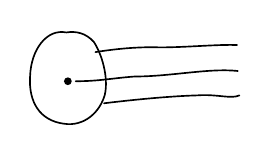
\begin{tikzpicture}[x=.01cm,y=-.01cm,line width=.6pt,line cap=round,line join=round]
\draw (54,11) .. controls (29,6) and (9,33) .. (8,67)
 .. controls (6,99) and (20,123) .. (51,127)
 .. controls (77,131) and (97,112) .. (103,90)
 .. controls (108,68) and (99,38) .. (89,23)
 .. controls (79,12) and (67,9) .. (54,11);
\draw (91,36) .. controls (116,32) and (145,29) .. (173,30)
 .. controls (207,30) and (247,26) .. (271,27);
\draw (66,73) .. controls (96,73) and (113,69) .. (141,67)
 .. controls (187,67) and (236,56) .. (272,60);
\draw (102,101) .. controls (135,97) and (184,92) .. (220,91)
 .. controls (246,89) and (263,96) .. (274,91);
\fill (56,73) circle (1.4pt);
\end{tikzpicture}}

On prend alors un voisinage tubulaire standart
\inserted{$T(S\dot T'_{ij})$} de $S\dot T'_{ij}$ dans $\dot T'_{ij}$,
% One live de stands below the formula's curved insertion leader; no separate cancelled duplicate is isolated.
% The S is reworked; tiny detached dark traces below-left of the following T stem are retained as a local reworking observation, with no invented glyph.
qu'on peut supposer induit par la réunion \inserted{$\bigcup T_k$}
des voisinages tubulaires standart des $X_k$ ($i<k<j$)
dans $\unsure{X\mathbin{\cdot-}X_j|X-X_j}$
% Between the two X groups a detached low dot/short oblique mark precedes one horizontal dash. Its role is uncertain.
(pris ``assez petits'' p.r. aux choix déjà faits de $T_{<i}$
et \inserted{de} $T'_{ij}$).
On \deleted{\unsure{prendra}}\inserted{aura} alors
\[
(43)\qquad\Sigma_{ij}=\dot T'_{ij}\setminus\mathring T(S\dot T'_{ij})
\]
% Pale foliation at the lower left, in another hand; the final display touches the paper edge.
\margin{72}

\scanpage{75}
\mspage{33}
On choisit un voisinage tubulaire \unsure{standard|standart} $T_{(0)}$ de
$X_{(0)}$ dans $X$, et on pose
\[
\begin{aligned}
\deleted{(\unsure{48})}\qquad&
\left\{\begin{aligned}
X^{(1)}_{\deleted{\unsure{i}}}&=X\setminus\mathring T_{(0)}\\
X^{(1)}_{(d)}&=X^{(1)}\cap X_{(d)}\qquad(=\varnothing\text{ si }d\leq0)
\end{aligned}\right.\\
&\quad X^{(1)}_i=X^{(1)}\cap X_i
\qquad\text{de sorte que}\quad
X^{(1)}_{(d)}=\bigcup_{\substack{i\in I\\\delta(i)\leq d}}X^{(1)}\cap X_i
\end{aligned}
\]
% The brace ends above the body of the third row; that row and its right continuation are unbraced.

On \deleted{pose}\inserted{prend} alors un voisinage tubulaire
standart \deleted{de} $T_1^{\unsure{\deleted{1}|1}}$ de $X_{(1)}$ dans $X$
(petit par rapport au choix de $T_0$), soit $T_1^{(1)}$ sa trace dans
$X^{(1)}$, qui est un vois. tub. standart de $X^{(1)}_{(1)}$ dans
$x^{(1)}$. On pose
\[
\deleted{(\unsure{49})}\qquad
\begin{aligned}
X^{(2)}&=X^{(1)}\setminus\mathring T^{(1)}_{(1)}
=X^{(1)}\cap(X\setminus\mathring T_1)\\
&=X^{\deleted{\unsure{2}}}\setminus(\mathring T_0\cup\mathring T_1)
\end{aligned}
\]
\margin{OPS $T_d=\displaystyle\bigcup_{\substack{i\in I\\\delta(i)\leq d}}T_i$,
où $T_i$ est un vois. tub. de $X_i$ dans $X$}
% The oblique note lies to the left of the second display and the following paragraph.

On prend un voisinage tubulaire $T_d$ de $X_{(d)}$ dans $X$,
petit p.r. aux vois. tubulaires $T_{d'}$ ($d'<d$) déjà construits,
et on pose
\[
(48)\qquad X^{(d)}=X-\bigcup_{\alpha<d}\mathring T_\alpha.
\]
% Two tiny isolated points below the equality are recorded as unassigned marks in the audit record.
Ceci posé, on pose, pour $i\in I$, $d=\delta(i)$
\[
(\unsure{49|41})\qquad|\quad
\begin{aligned}
\Sigma_i&=X_i\cap X_{(d)}
=X_i\setminus\deleted{\unsure{\{}}\bigcup_{\underline{\alpha}<d}X_i\cap
\unsure{\dot T_\alpha|\mathring T_\alpha}
\qquad\deleted{\unsure{\subset X_i|\cap X_i}}\\
&=X_i\setminus\bigcup_{\underset{\sim}{j}<i}X_i\cap\mathring T_j
\qquad\subset X_i^*
\end{aligned}
\]
% The isolated upright before Sigma has no assigned mathematical function here.
\margin{74}
% Foliation in another, unnamed hand at the lower left.

\scanpage{76}
Si $i<j$, \deleted{$d=\delta(i),\ d'=\delta(j)$}
\[
(49)\qquad\Sigma_{ij}=\deleted{\unsure{\dot T_j|\dot T_{ij}}\cap\Sigma_j}
\dot T_i\cap\Sigma_j\quad\subset\Sigma_j
\]
et pour un drapeau $i_0<i_1--<i_n$
\[
(50)\qquad\begin{aligned}
\Sigma_{i_0.--i_n}&=\dot T_{i_0}\cap\dot T_{i_1}\cap .-\cap
\dot T_{i_{n-1}}\cap\Sigma_{i_n}\\
&=\Sigma_{i_0i_n}\cap\Sigma_{i_1i_n}.--\cap\Sigma_{i_{n-1}i_n}
\end{aligned}
\]
% The continuation clusters are local written shapes: two short strokes in
% the flag; point plus two strokes in the first Sigma index and second row;
% point plus one stroke in the first row.
On a \inserted{de façon évidente} les morphismes de transition
\inserted{entre les $\Sigma_{i_0--i_n}$} pour les
\deleted{\unsure{morphismes}} inclusions \uline{cofinales} de drapeaux,
mais non pour des inclusions quelconques, dont la définition dépend
du choix de rétractions des
\[
T_i^{(d)}=T_i\cap X^{(d)}\qquad d=\delta(i)
\]
sur $X_{\unsure{i|j}}^{(d)}=X_i\cap X^{(d)}$, ce qui donne alors
\deleted{\unsure{f|t}}
\[
\Sigma_{ij}\subset\dot T_i^{(d)}\subset T_i^{(d)}
\longrightarrow X_i^{(d)}=\Sigma_i
\]
la structure complète
\diagram{\begin{tikzcd}[column sep=large,row sep=small]
&&\Sigma_j&\\
((\Sigma_i),(\Sigma_{ij}),&\Sigma_{ij}\arrow[ur]\arrow[dr]&&\unsure{\Bigg)}\\
&&\Sigma_i&
\end{tikzcd}}
% Only the upper and lower ends of the outer closing parenthesis survive
% at the right paper edge; its middle continuation is cut off.

(Mais il faut des hyp. d'équisingularité sur la
\deleted{\unsure{fib|f}} stratification de $\unsure{\alpha|X}$ par les $X_i$,
et une condition \inserted{de \unsure{locale} trivialité}
sur les rétractions
$T_i^{(d)}\longrightarrow X_i$ i.e. \inserted{sur les}
$T_{(d)}^{(d)}\longrightarrow X_{(d)}^{(d)}$,
pour que les $\Sigma_{ij}\mathrel{-}\Sigma_i$ soient des fibrations)

....
% A separate much lower-left dark speck is visible below the four aligned
% continuation points; its function is unassigned.
\margin{\handwritten{75}}

\scanpage{77}
\mspage{34}
\uline{15}. Introduction des proespaces :
${\unsure{V|\mathcal V}}_{i_0.\!-.i_n},\ {\unsure{V|\mathcal V}}_J^{\deleted{\unsure{*}}L}$,
% The title has a dot, a short horizontal dash, and a dot between the indices.
% Both V forms have a curved bowl; plain/calligraphic alphabet assignment remains open.

On désigne par ${\unsure{V|\mathcal V}}_i^{\unsure{*|<|\deleted{*}}}$
\unsure{\deleted{le}|le} \inserted{pro}voisinage tubulaire
(au sens des proespaces) de $X_i^*=X_i\setminus\bigcup_{j<i}X_j$
dans $X$. Ainsi, \deleted{\unsure{on}} \unsure{on a}
% The raised pro has a curved leader ending immediately before voisinage.
\[
(51)\qquad X_i^*\longrightarrow {\unsure{V|\mathcal V}}_i^{\unsure{*|\deleted{*}}}
\qquad\begin{gathered}
\text{équivalence d'homo-}\\
\text{topie \unsure{des|de} proespaces.}
\end{gathered}
\]
% The hyphen after homo is written at the right paper edge.

\deleted{\unsure{Pour un drapeau}}
Si\unsure{)} $i<j$, on pose
% The separate curved stroke after Si is retained; no opening parenthesis is supplied.
\[
(52)\qquad
\unsure{\rlap{$X$}V|\rlap{$X$}\mathcal V}_{ij}={\unsure{V|\mathcal V}}_i\cap {\unsure{V|\mathcal V}}_j
\]
% The left base in (52) is one superposed X/V cluster with a single shared ij.
% The overprinting order and deletion state cannot be separated; no second index is supplied.

\margin{Pour un
\diagram{\begin{tikzcd}[column sep=small]
{\unsure{V|\mathcal V}}_{ij}^{\unsure{b}}={\unsure{V|\mathcal V}}_i\cap X_j^*\arrow[r,hook]&{}
\end{tikzcd}}
est-ce une équivalence d'homotopie ?}
% The oblique left note ends its formula at the curved arrowhead; no target letters are visible.

\margin{NB ${\unsure{V|\mathcal V}}_{ij}$ a un sens \deleted{\unsure{si}} si $i\neq j$
mais si $i$ et $j$ ne sont pas comparables, on a
${\unsure{V|\mathcal V}}_i\cap {\unsure{V|\mathcal V}}_j=\varnothing$,
\inserted{(du moins si les ouverts de $X$ sont normaux, p.ex. $X$ métrisable)}
si $i=j$, on a ${\unsure{V|\mathcal V}}_{ii}={\unsure{V|\mathcal V}}_i$}
% The long curved leader joins the parenthetical insertion to the intersection-empty clause.
% The parenthetical words are physically below V_ii=V_i; their attachment precedes si i=j.

de sorte qu'on a
\diagram{\begin{tikzcd}[column sep=large,row sep=huge]
&{\unsure{V|\mathcal V}}_{ij}\arrow[r,hook,"b_{ij}"]\arrow[d,hook,"s_{ij}"]&{\unsure{V|\mathcal V}}_j\\
\Bigl(X_i
\arrow[r,shift right=1.2ex]
\arrow[r,phantom,"{\substack{\unsure{(w)|(h)}\\\sim\\
\unsure{\longleftarrow|\deleted{\longleftarrow}}}}"]
&\Bigr){\unsure{V|\mathcal V}}_i&
\end{tikzcd}}
% Four written connectors: two hooked main arrows, the dense left-pointing lower mark,
% and a separate lower right-pointing arrow. The left-pointing mark has unresolved strike state.
% The closing parenthesis lies before V_i, with the one tilde and (w)/(h) above the lower marks.
On a :
\[
(53)\qquad X=\varinjlim\bigl({\unsure{V|\mathcal V}}_i,{\unsure{V|\mathcal V}}_{ij},
\unsure{\deleted{\}}|\}}\ b_{ij},s_{ij}\bigr)
\]
% The brace-like glyph between the comma and b is crossed/reworked; its strike state remains open.
$X$ est obtenu par \uline{recollement} des ${\unsure{V|\mathcal V}}_i$
suivant les ${\unsure{V|\mathcal V}}_{ij}$.

On définit aussi, plus généralement, les
\[
(54)\qquad {\unsure{V|\mathcal V}}_{i_0.\!-i_n}={\unsure{V|\mathcal V}}_{i_0}\cap
\mathord{-}\,\mathord{-}\cap {\unsure{V|\mathcal V}}_{i_n}
\]
% The left index has dot-dash; the right continuation has two separate dashes.
% The final V is retraced, without a recoverable independently cancelled underlying letter.
pour un drapeau $i_0<i_1<.\!-<i_n$
\margin{\uline{NB} L'expression a un sens $=$ si
l'ens. $\{i_0,\mathord{-}i_n\}$ ne forme pas un drapeau,
mais il est vide si ce n'est pas un drapeau}
% The bottom marginal note is oblique. Its = has two horizontal strokes, the lower slightly wavy.
% The continuation within the written braces is one dash, with no second comma before i_n.
% Pale bottom-left foliation in another, unnamed hand:
\margin{76}

\scanpage{78}
c'est un système inductif de \deleted{\unsure{espaces}} proespaces
sur l'ens ordonné opposé de celui des drapeaux de $I$
(\unsure{pour|avec} l'inclusion), dont le $\uline{\lim}$ est égalt $\approx X$.

Soit $Z$ \deleted{$X$} une partie (\inserted{loc\textsuperscript{t}} fermée)
de $X$, et posons, pour \deleted{$\unsure{\forall}$} un $i$ tel que
${\unsure{\deleted{{\unsure{V|\mathcal V}}}X|\deleted{X}{\unsure{V|\mathcal V}}}}_i^{\unsure{*}}
\subset\unsure{\deleted{X}Z|\deleted{Z}X}$
% The two overwritten base glyphs at each end remain in uncertain layer order.
% One shared low i and the crowded raised star-candidate are retained at the left.
\[
(55)\qquad {\unsure{V|\mathcal V}}_i^Z
={\unsure{V|\mathcal V}}_i\cap Z\qquad
\begin{gathered}
\text{provoisinage tubulaire}\\
\text{de }X_i^*\text{ dans }Z
\end{gathered}
\]
\deleted{\unsure{de|et}}
on a
\[
(56)\qquad X_i^*\hookrightarrow
{\unsure{V|\mathcal V}}_i^{\unsure{2|Z}}\hookrightarrow{\unsure{V|\mathcal V}}_i
\qquad\begin{gathered}
\text{équivalences}\\
\text{d'homotopie}
\end{gathered}
\]
Plus \unsure{généralt}, on pose (si $X_{i_n}\subset Z$)
\[
{\unsure{V|\mathcal V}}_{i_0-i_n}^Z
={\unsure{V|\mathcal V}}_{i_0-i_n}\cap Z
={\unsure{V|\mathcal V}}_{i_0}^Z\cap\cdot-\cap{\unsure{V|\mathcal V}}_{i_n}^Z
\]
C'est aussi le ${\unsure{V|\mathcal V}}_{i_0--i_n}$ relatif : le \deleted{\unsure{fil}}
stratificati\unsure{-}
% A short terminal baseline stroke reaches the right paper edge; no unseen ending is supplied.
de $Z$ induite par les
$Z_i\overset{\mathrm{def}}{=}X_i\cap Z$, pour le système d'indices
$i_0--i_n$. On a
\[
(57)\qquad {\unsure{V|\mathcal V}}_{i_0\cdot--i_n}^Z
\hookrightarrow{\unsure{V|\mathcal V}}_{i_0--i_n}
\qquad\text{\unsure{équiv.|équiv} d'homotopie}
\]
% Two tiny isolated points near the raised Z are recorded without an assigned role.
Soit $J$ une partie de $I$, posons
\[
(58)\qquad X_J^*=\bigcup_{i\in J}X_i^*,\qquad X_J=\bigcup_{i\in J}X_i
\]
\margin{77}
% Foliation in another unnamed hand at the lower left; no author number is visible.
